\documentclass{article}
\usepackage{geometry}
\usepackage{longtable}
\usepackage{array}

\usepackage{graphicx}
\usepackage{listings}
\usepackage{hyperref}
\usepackage{float}

\lstset{
  basicstyle=\ttfamily,
  columns=fullflexible,
  breaklines=true
}

\newcommand{\modelentry}[1]{%
  \begin{figure}[H]
    \centering
    \includegraphics[width=\textwidth]{images/exported_bpmn/#1.pdf}
    \caption{Model: \detokenize{#1}}
    \label{fig:#1}
  \end{figure}
}

\AtBeginDocument{%
  \immediate\write18{./bpmn_to_image.sh}%
}

\geometry{
  left=1in,
  right=1in,
  top=0.5in,
  bottom=0.5in
}

\title{MSP Report - Sprint 2}
\author{Franka Traupe, Roschanak Babai, Niklas Sander, Valeriia Baida, Guilherme Fernandes}
\date{}

\begin{document}

\maketitle

\textbf{Github (Sprint 1):} \url{https://github.com/niklassander/MSP/releases/tag/Sprint1_Submission}

\textbf{Github (Sprint 2):} \url{https://github.com/niklassander/MSP/releases/tag/Sprint2_Submission}

\section*{Roles}
\textbf{Scrum Master:} Franka Traupe\\
\textbf{Product Owner:} Guilherme Fernandes\\
\textbf{Quality Controllers and Development Team:} Franka Traupe, Guilherme Fernandes, Roschanak Babai, Valeriia Baida, Niklas Sander\\

\section*{Features}
(Implemented features highlighted in bold)

\subsection*{Basic Features (Implemented in prototype)}
\begin{itemize}
    \item \textbf{Register account}
    \item \textbf{Register type of vehicle}
    \item \textbf{Define route}
    \item \textbf{Alert if speed limit is violated}
    \item \textbf{Calculate estimated time of arrival}
\end{itemize}

\subsection*{Features from Existing System}
\begin{itemize}
    \item \textbf{Bookmarking (home, work, custom)}
    \item Avoid tolls
    \item \textbf{Recent destinations}
    \item Show current speed (implemented already as part of speed alerts)
    \item Parking lots
    \item \textbf{Hazard reports}
    \item \textbf{Change units}
\end{itemize}

\subsection*{New Features}
\begin{itemize}
    \item \textbf{Statistics: usage and driving quality (distance traveled, active days etc.)}
    \item Walking route
    \item Shared ride
\end{itemize}

\section*{Project Planning: Sprint 1}

\subsection*{Task Table}

\begin{table}[H]
  \centering
  \begin{tabular}{|c|p{6cm}|c|c|}
  \hline
  \textbf{Task ID} & \textbf{Task} & \textbf{Duration (days)} & \textbf{Depends on} \\
  \hline
  1 & Explore original app \& choose features & 3 & - \\
  2 & Review chosen features & 1 & 1 \\
  3 & Develop BPMNs for each feature & 4 & 2 \\
  4 & Review BPMNs & 1 & 3 \\
  5 & Front-end development & 7 & 4 \\
  6 & Back-end development & 7 & 4 \\
  7 & Integrate front-end and back-end & 2 & 5,6 \\
  8 & Testing & 2 & 7 \\
  9 & Bug Fixing & 1 & 8 \\
  \hline
  \end{tabular}
  \caption{Task List with Dependencies}
  \label{tab:tasklist}
\end{table}

\subsection*{Gantt Chart}

\begin{figure}[H]
  \centering
  \includegraphics[width=\textwidth]{images/gantt_chart.png}
  \caption{Gantt Chart}
  \label{fig:gantt_chart}
\end{figure}

\subsection*{Burndown Chart}

\begin{figure}[H]
  \centering
  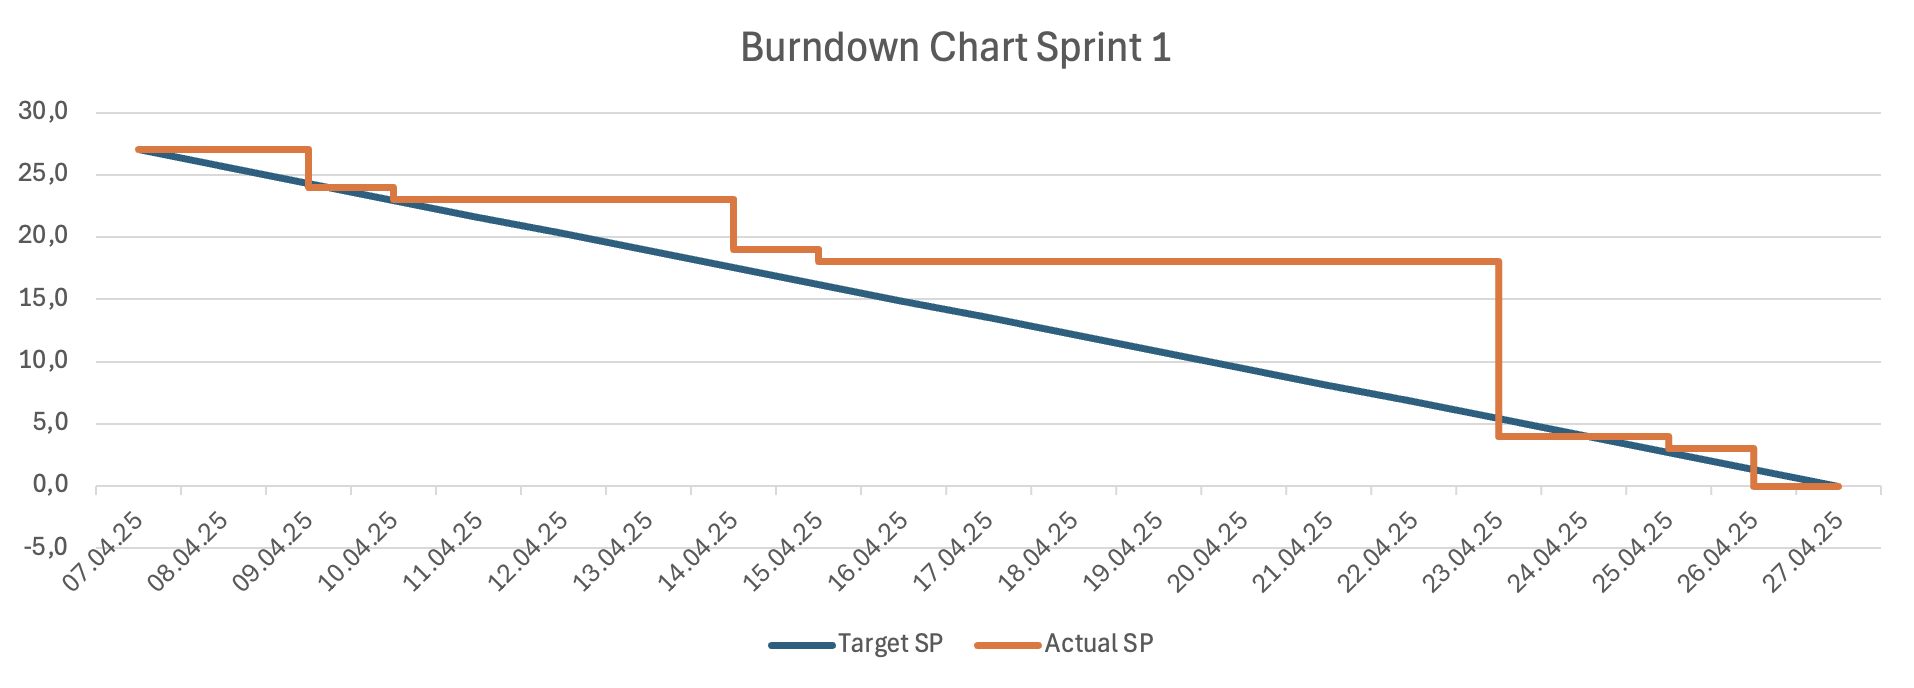
\includegraphics[width=\textwidth]{images/burndown.png}
  \caption{Burndown Chart}
  \label{fig:burndown_chart}
\end{figure}

  
\clearpage

\section*{Project Planning: Sprint 2}

\subsection*{Task Table}

\begin{table}[H]
  \centering
  \begin{tabular}{|c|p{6cm}|c|c|}
  \hline
  \textbf{Task ID} & \textbf{Task} & \textbf{Duration (days)} & \textbf{Depends on} \\
  \hline
  1 & Sprint 1 Revision & 2 & - \\
  2 & Context Diagram & 3 & 1 \\
  3 & Use Case View & 3 & 1 \\
  4 & Logical View & 3 & 1 \\
  5 & Development View & 4 & 4 \\
  6 & Process View & 11 & 5 \\
  7 & Prototyping & 11 & 5 \\
  8 & Deployment View & 3 & 7 \\
  \hline
  \end{tabular}
  \caption{Task List with Dependencies}
  \label{tab:tasklist2}
\end{table}

\subsection*{Gantt Chart}

\begin{figure}[H]
  \centering
  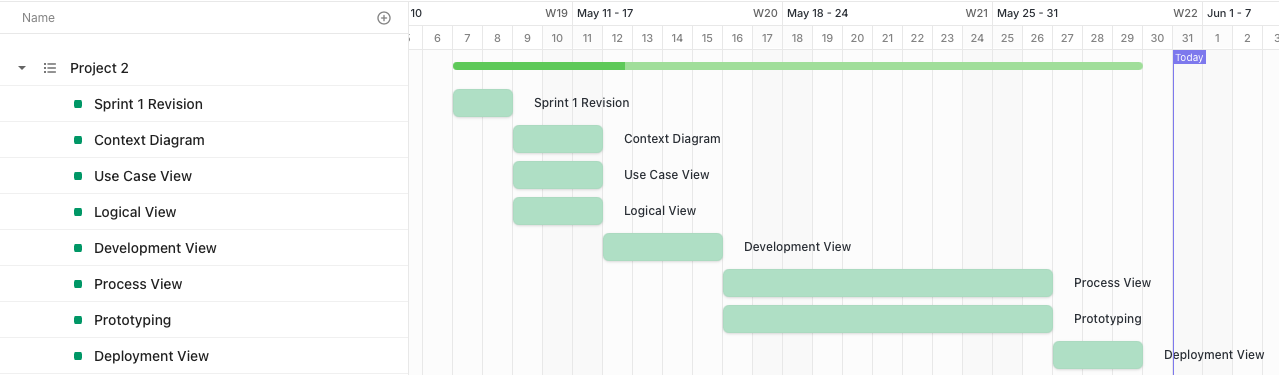
\includegraphics[width=\textwidth]{images/gantt2.png}
  \caption{Gantt Chart}
  \label{fig:gantt_char2}
\end{figure}

\subsection*{Burndown Chart}

\begin{figure}[H]
  \centering
  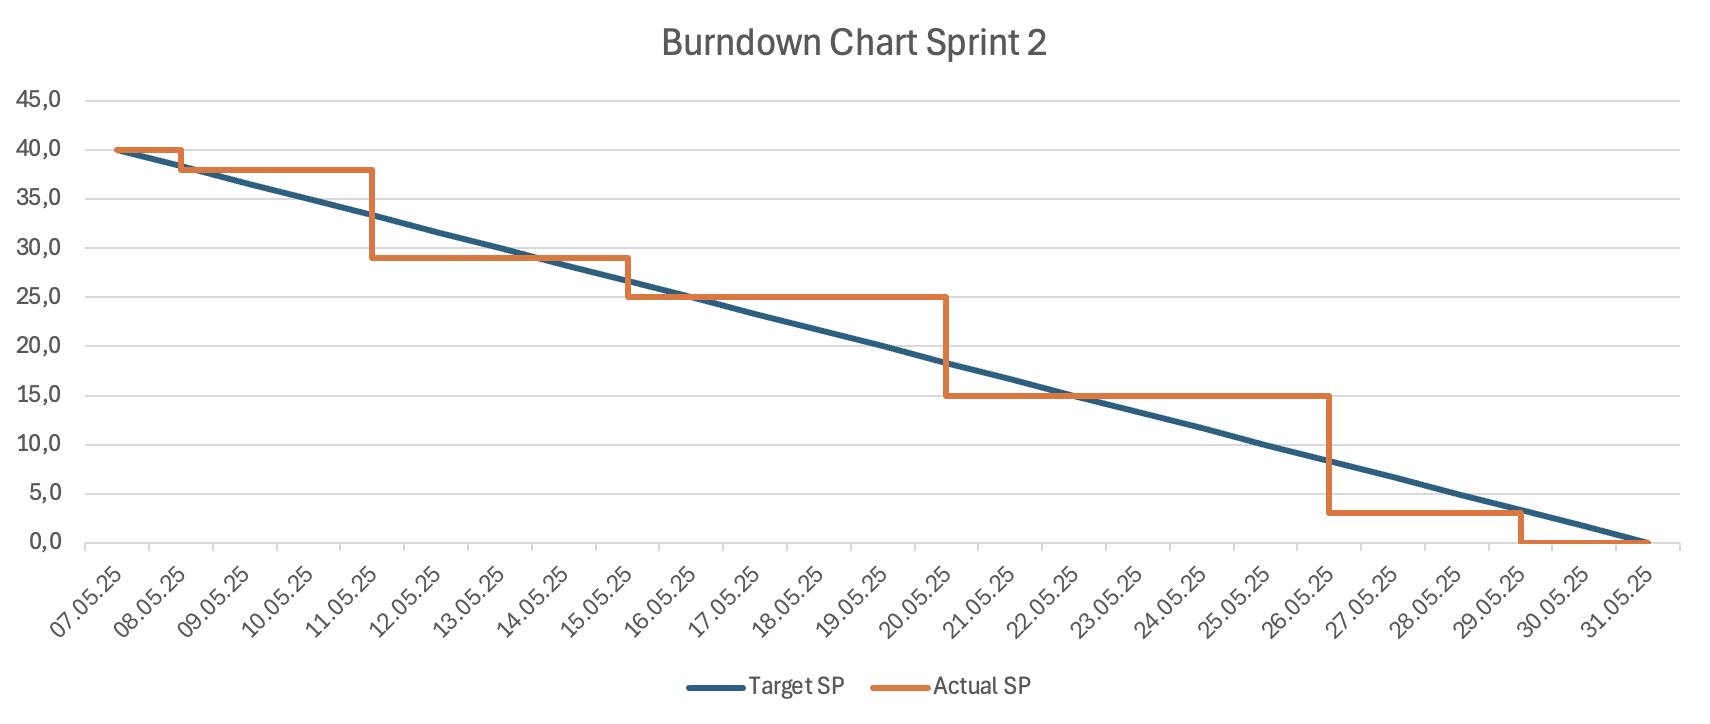
\includegraphics[width=\textwidth]{images/burndown2.png}
  \caption{Burndown Chart}
  \label{fig:burndown_chart2}
\end{figure}

\clearpage

\section*{Requirements Diagrams}
\begin{figure}[H]
    \centering
    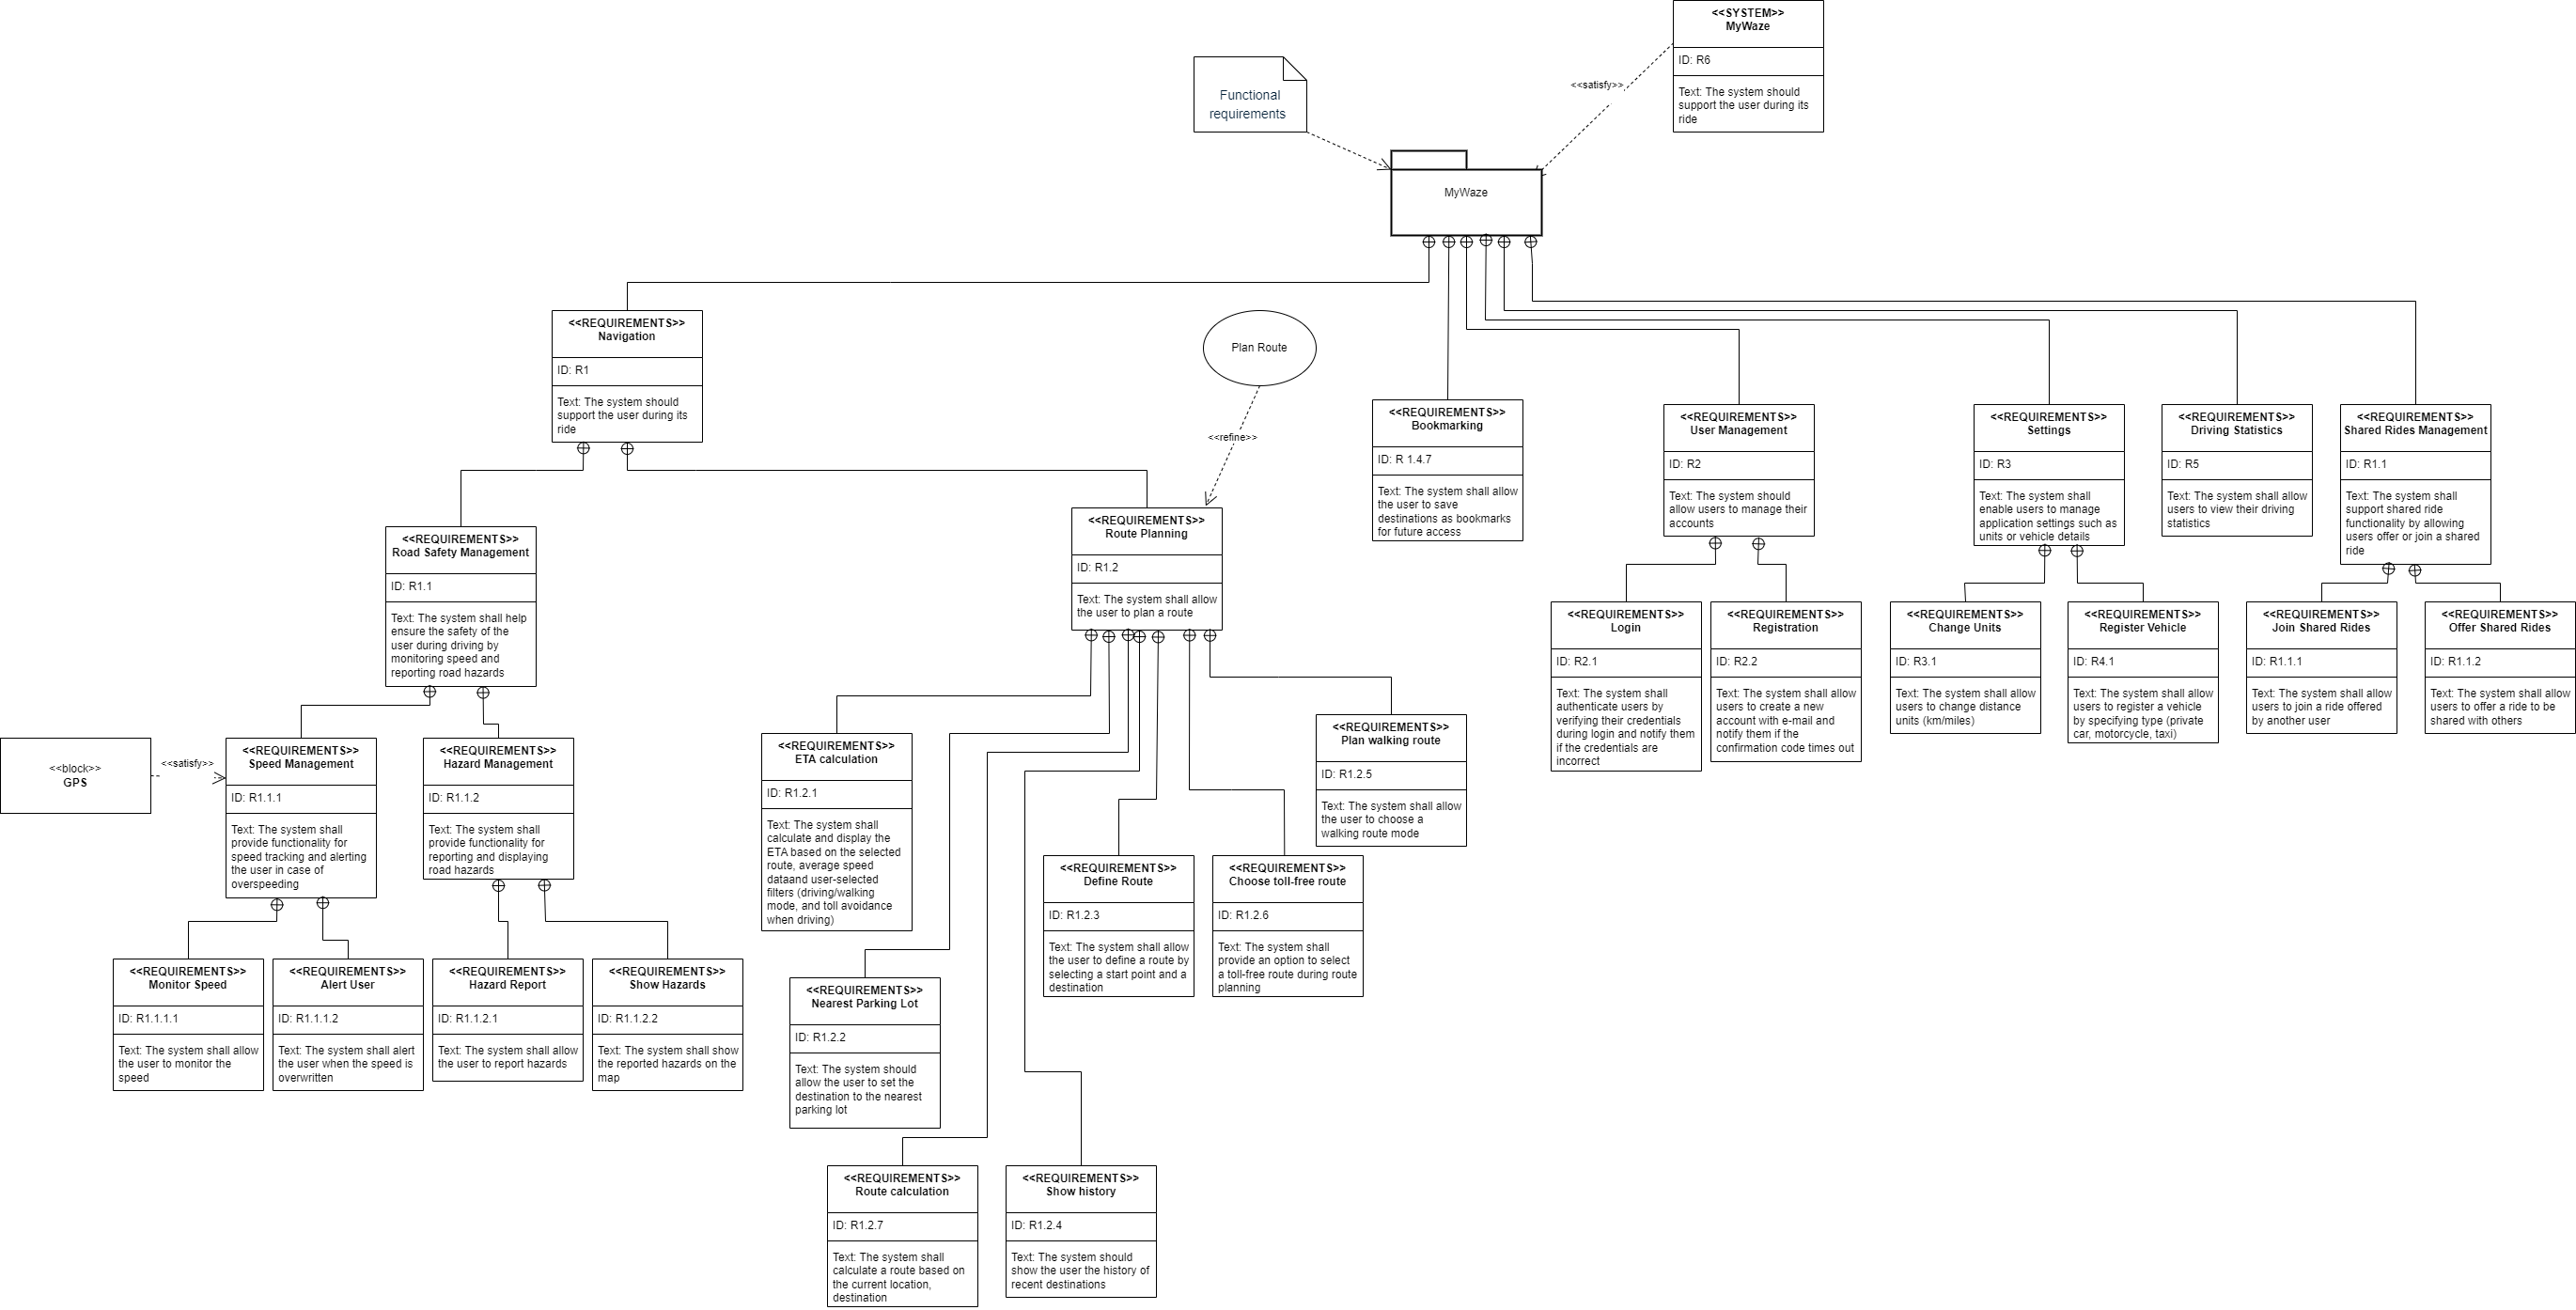
\includegraphics[width=\textwidth]{images/SysML_MyWaze_FR.drawio.png}
    \caption{Functional Requirements}
    \label{fig:fr_requirements_diagram}
\end{figure}


\begin{figure}[H]
    \centering
    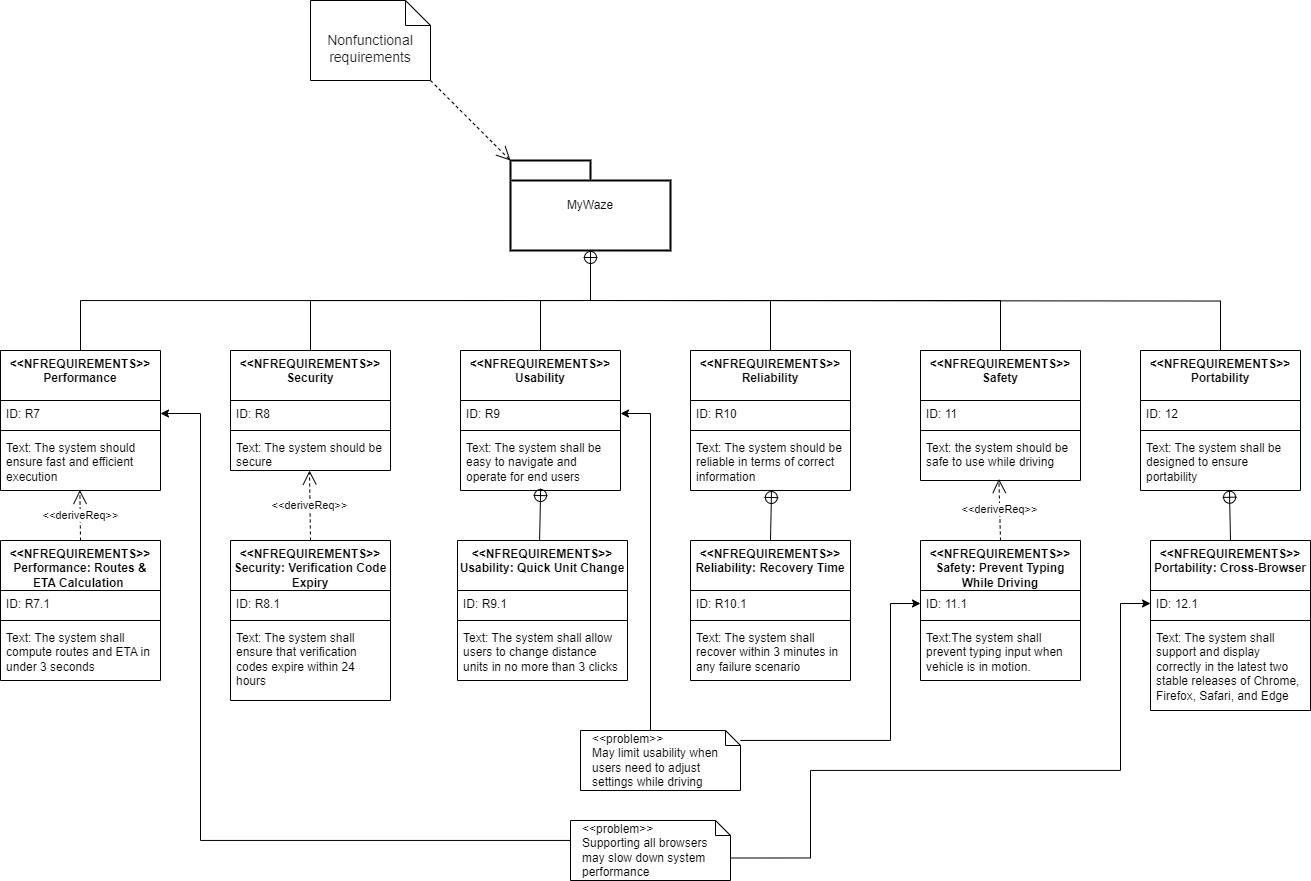
\includegraphics[width=\textwidth]{images/SysML_MyWaze_NFR.drawio.png}
    \caption{Nonfunctional Requirements}
    \label{fig:nfr_requirements_diagram}
\end{figure}

  
\clearpage

\section*{Mapping from Features to Models}

\begin{longtable}{|>{\raggedright}p{0.4\textwidth}|>{\raggedright\arraybackslash}p{0.5\textwidth}|}
\hline
\textbf{Feature} & \textbf{Model} \\
\hline
Overall process & MyWaze.bpmn \\
\hline
Register account & MyWaze\_registerAccount.bpmn \\
\hline
Recent destinations & MyWaze\_defineDestination.bpmn \\
\hline
Define route & MyWaze\_defineRoute.bpmn, MyWaze\_calculateRoute.bpmn \\
\hline
Avoid tolls & MyWaze\_defineRoute.bpmn \\
\hline
Walking route & MyWaze\_defineRoute.bpmn \\
\hline
ETA & MyWaze\_defineRoute.bpmn \\
\hline
Current speed & MyWaze\_navigate.bpmn, MyWaze\_speedMonitoring.bpmn \\
\hline
Speed alert & MyWaze\_navigate.bpmn, MyWaze\_speedMonitoring.bpmn \\
\hline
Find parking lots & MyWaze\_navigate.bpmn, MyWaze\_defineRouteToParkingLot.bpmn, MyWaze\_calculateRoute.bpmn \\
\hline
Hazard reports & MyWaze\_navigate.bpmn, MyWaze\_reportHazard.bpmn \\
\hline
Share ride & MyWaze.bpmn, MyWaze\_registerRideOffering.bpmn, MyWaze\_arrangeSharedRide.bpmn \\
\hline
Bookmarking & MyWaze.bpmn, MyWaze\_createBookmark.bpmn \\
\hline
Statistics & MyWaze.bpmn, MyWaze\_provideStatistics.bpmn \\
\hline
Change units & MyWaze.bpmn, MyWaze\_changeUnits.bpmn \\
\hline
Register vehicle type & MyWaze.bpmn, MyWaze\_registerVehicleType.bpmn \\
\hline
\end{longtable}

\section*{BPMN Models}
\input{models_list.tex}

\section*{Context Diagram}
\begin{figure}[H]
  \centering
  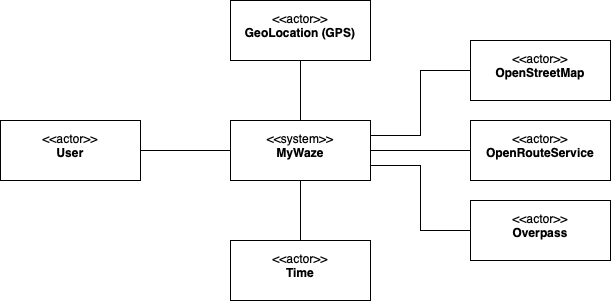
\includegraphics[width=\textwidth]{images/ContextDiagram.drawio.png}
  \caption{Context Diagram}
  \label{fig:contextDiagram}
\end{figure}

\section*{Use Case View}

\begin{figure}[H]
  \centering
  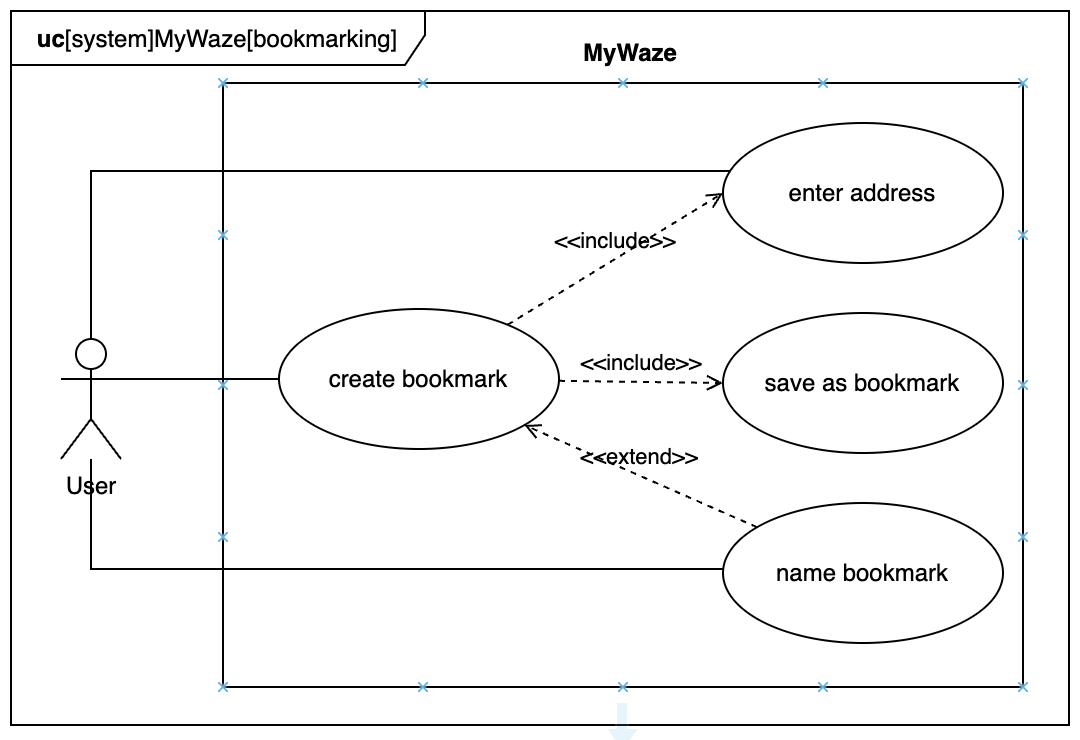
\includegraphics[width=\textwidth]{UseCases/Use_Case_Bookmarking.png}
  \caption{Use Case Diagram: Bookmarking}
  \label{fig:useCaseBookmarking}
\end{figure}

\begin{figure}[H]
  \centering
  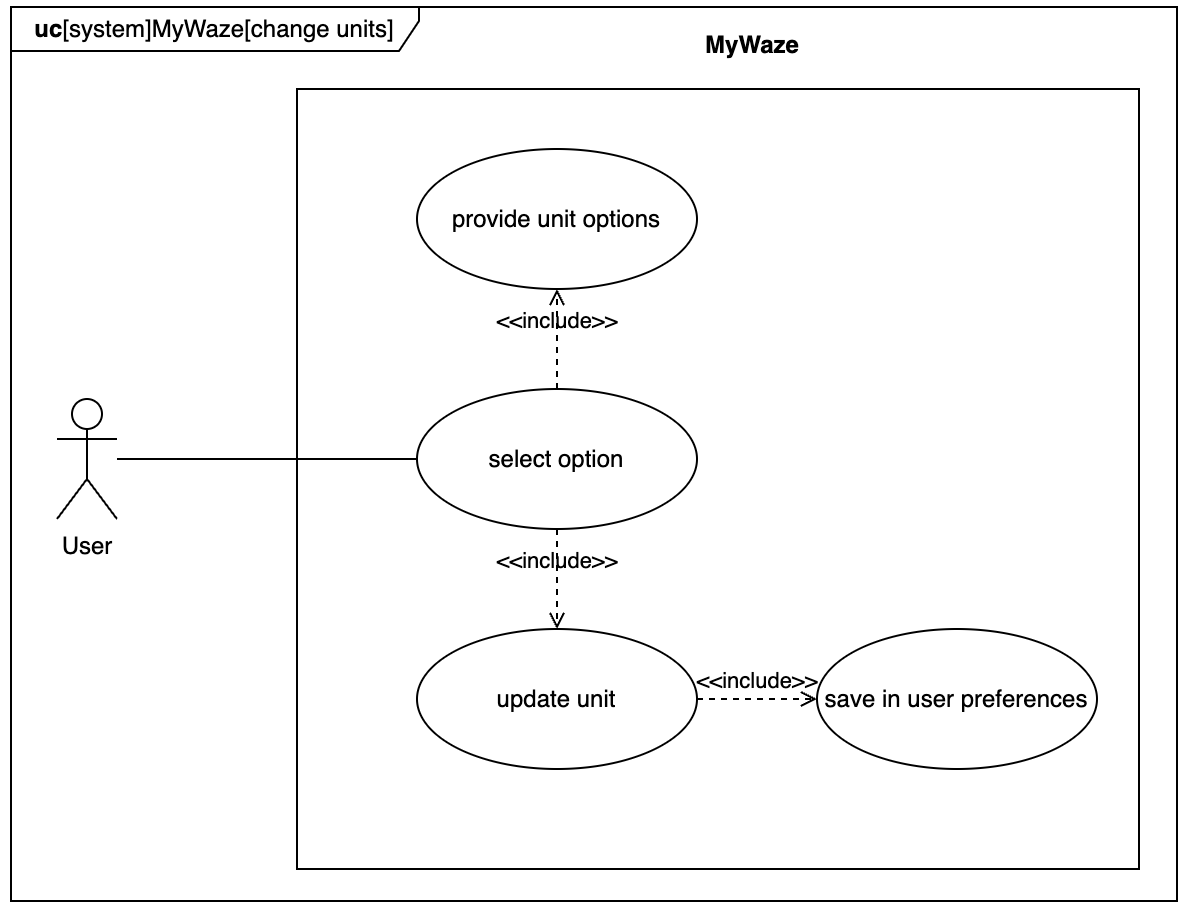
\includegraphics[width=\textwidth]{UseCases/Use_Case_Change_Units.png}
  \caption{Use Case Diagram: Change Units}
  \label{fig:useCaseChangeUnits}
\end{figure}

\begin{figure}[H]
  \centering
  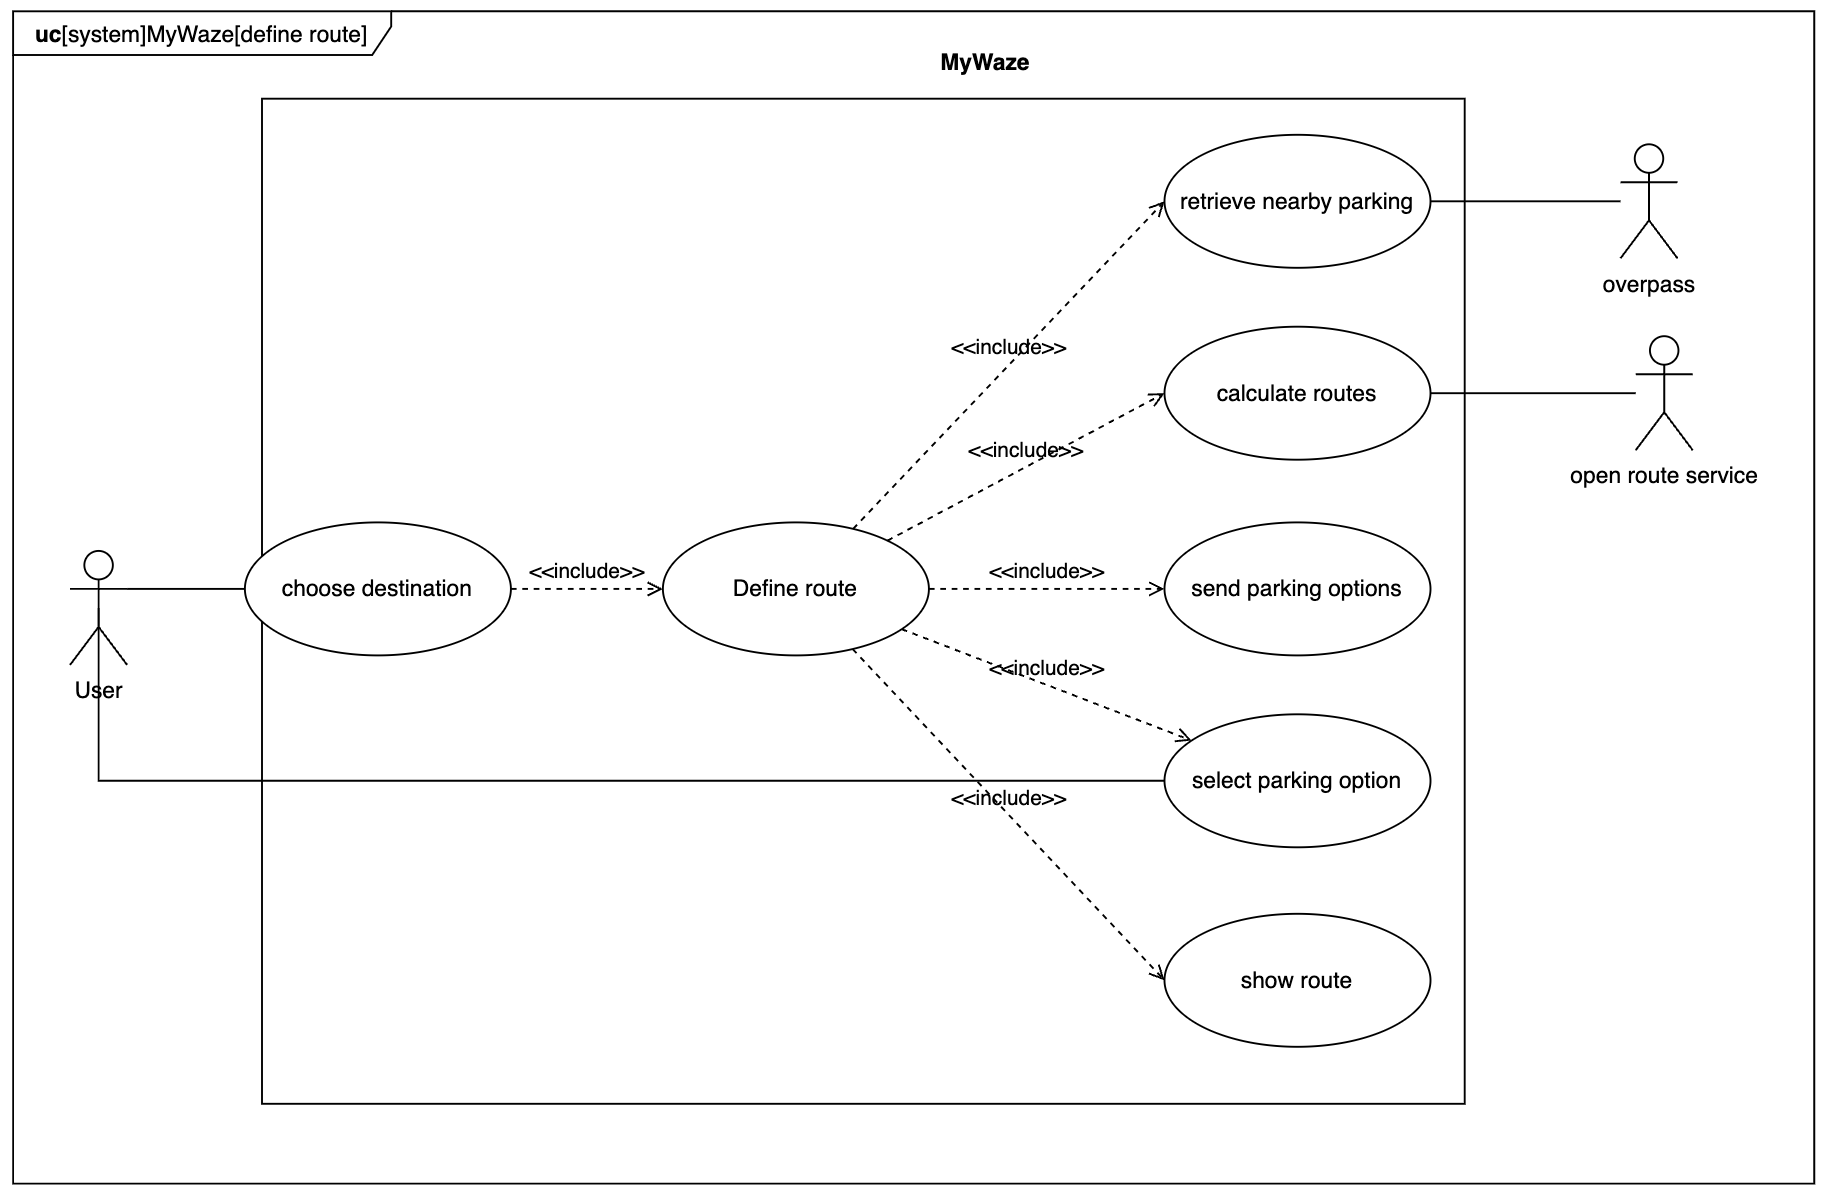
\includegraphics[width=\textwidth]{UseCases/Use_Case_Define_Route.png}
  \caption{Use Case Diagram: Define Route}
  \label{fig:useCaseDefineRoute}
\end{figure}

\begin{figure}[H]
  \centering
  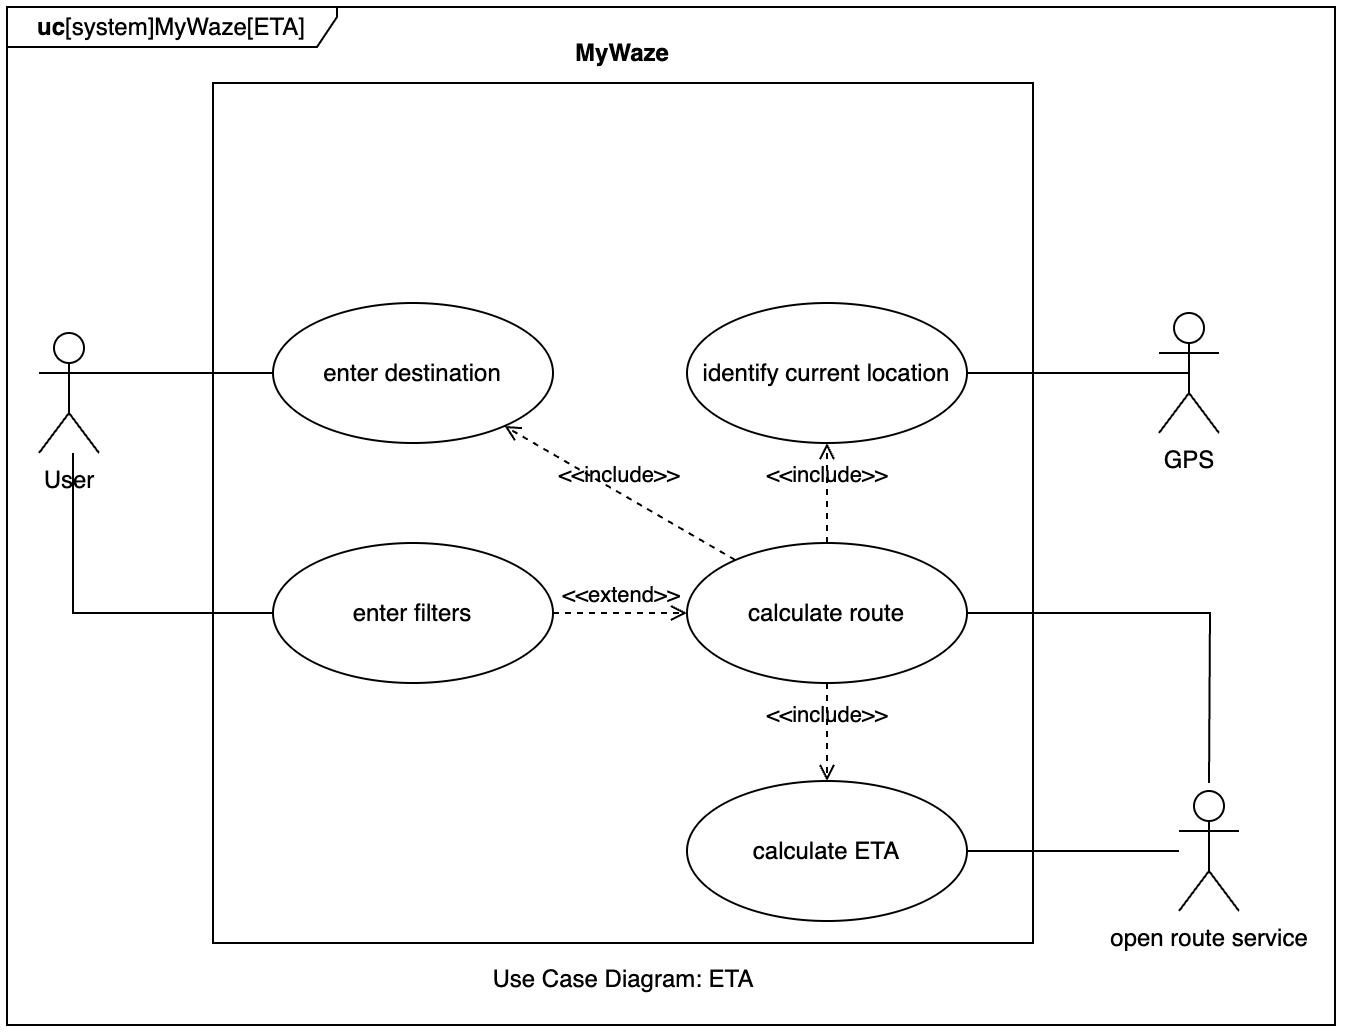
\includegraphics[width=\textwidth]{UseCases/Use_Case_ETA.png}
  \caption{Use Case Diagram: ETA}
  \label{fig:useCaseETA}
\end{figure}

\begin{figure}[H]
  \centering
  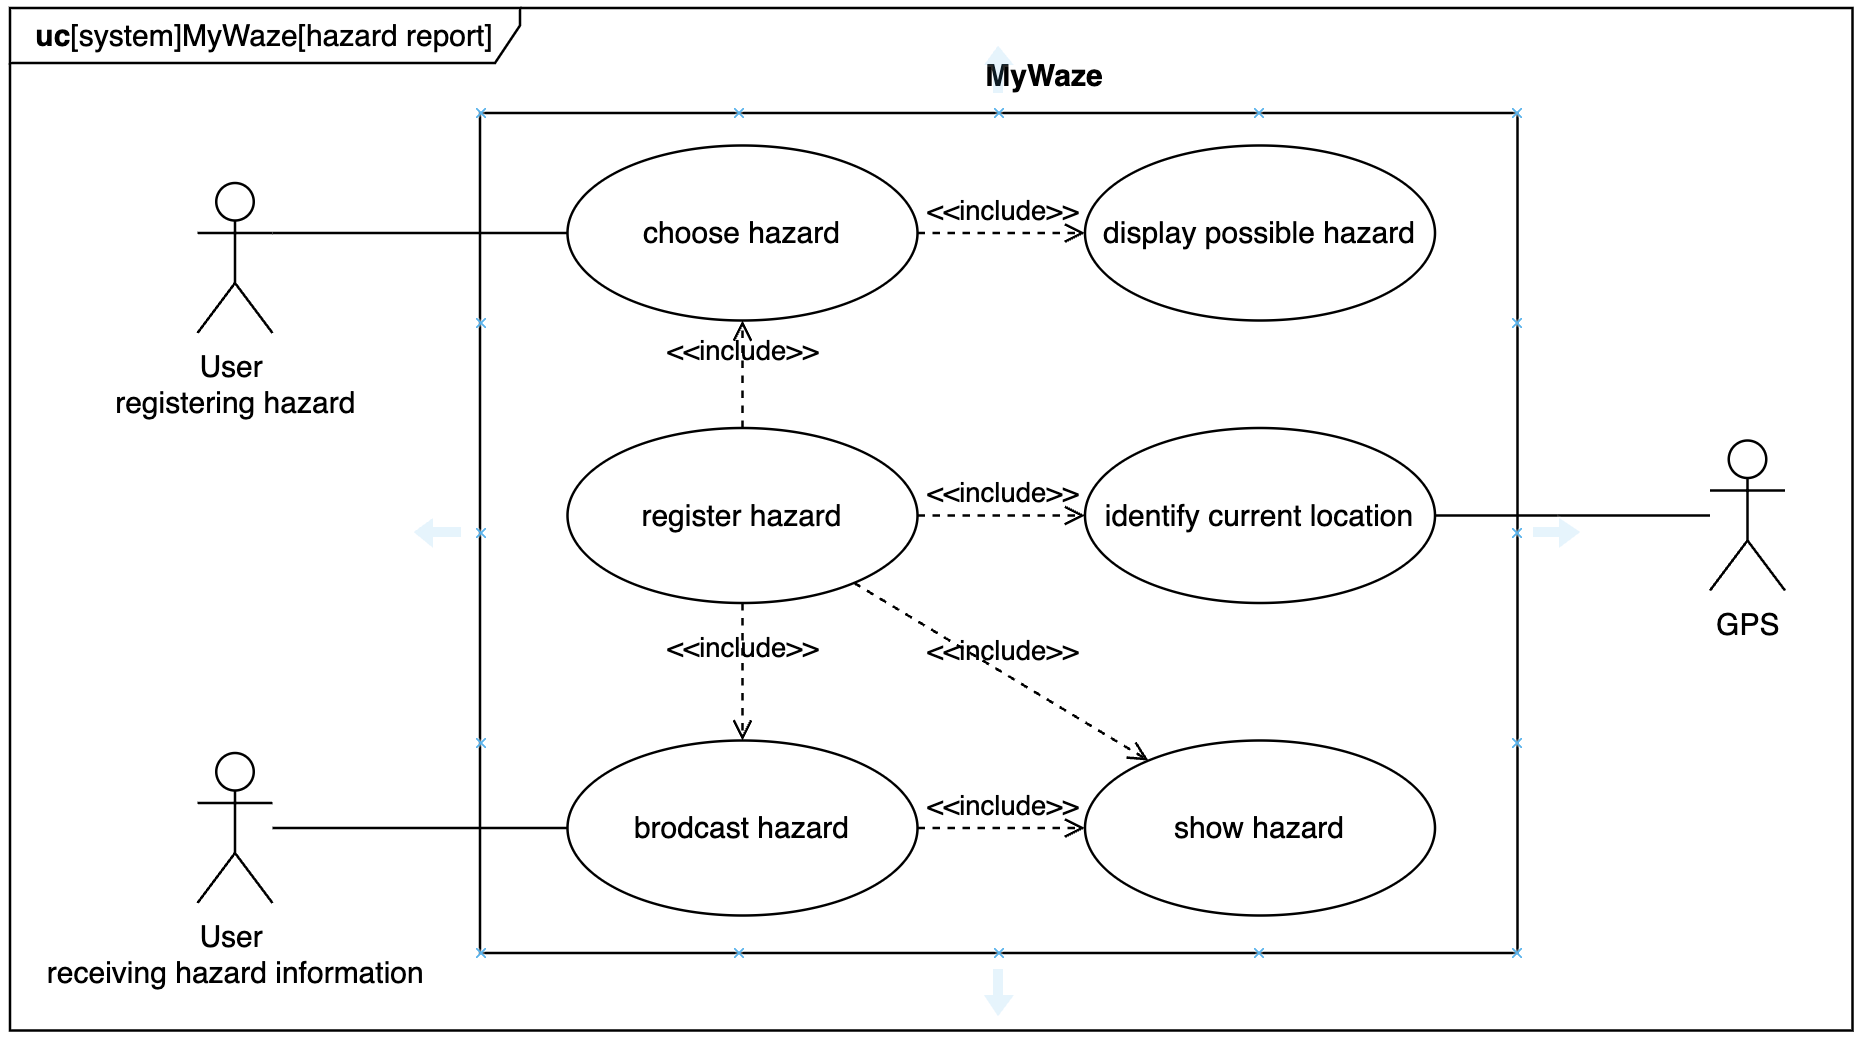
\includegraphics[width=\textwidth]{UseCases/Use_Case_Hazard_Report.png}
  \caption{Use Case Diagram: Hazard Report}
  \label{fig:useCaseHazardReport}
\end{figure}

\begin{figure}[H]
  \centering
  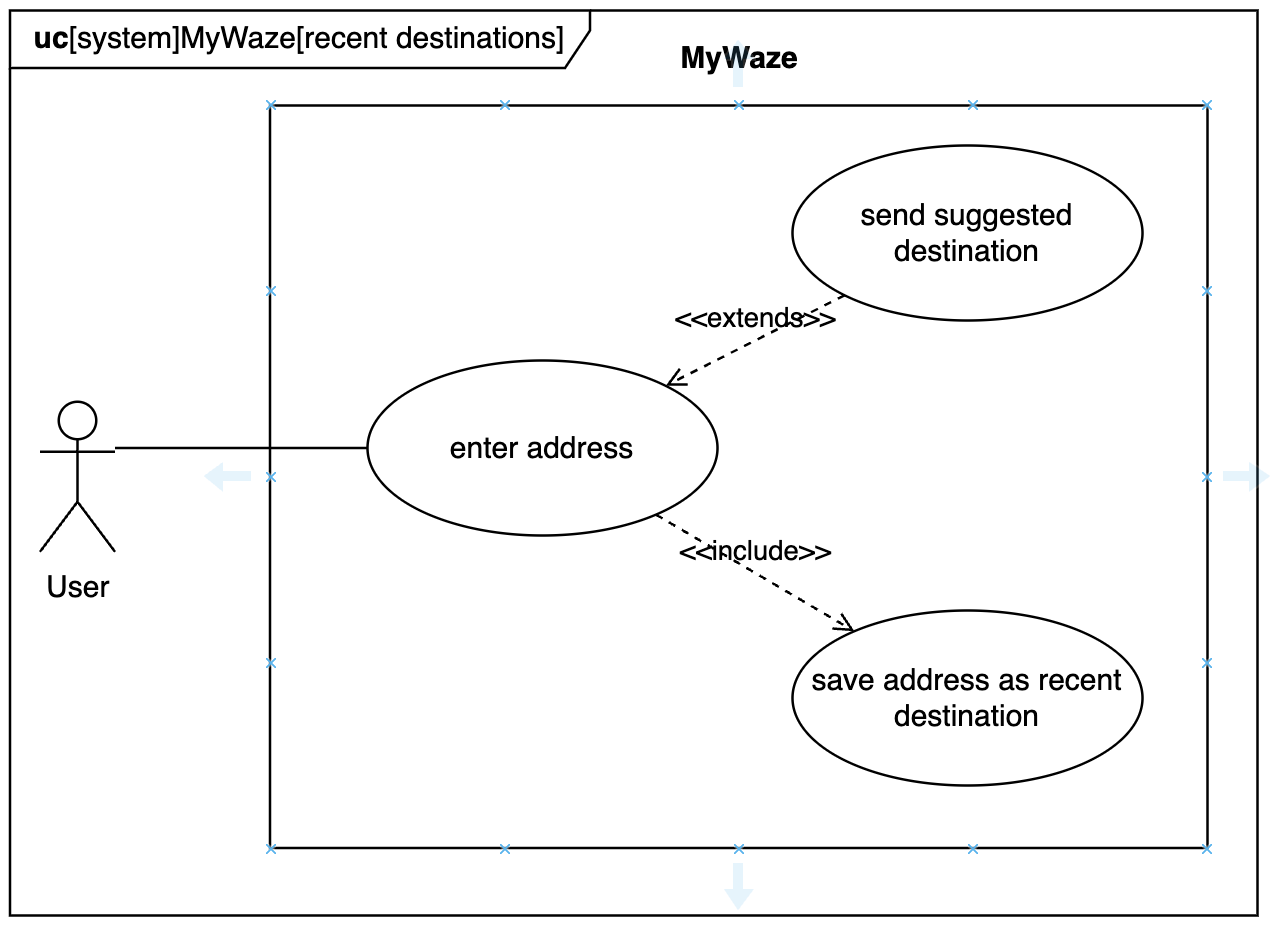
\includegraphics[width=\textwidth]{UseCases/Use_Case_Recent_Destinations.png}
  \caption{Use Case Diagram: Recent Destinations}
  \label{fig:useCaseRecentDestinations}
\end{figure}


\begin{figure}[H]
  \centering
  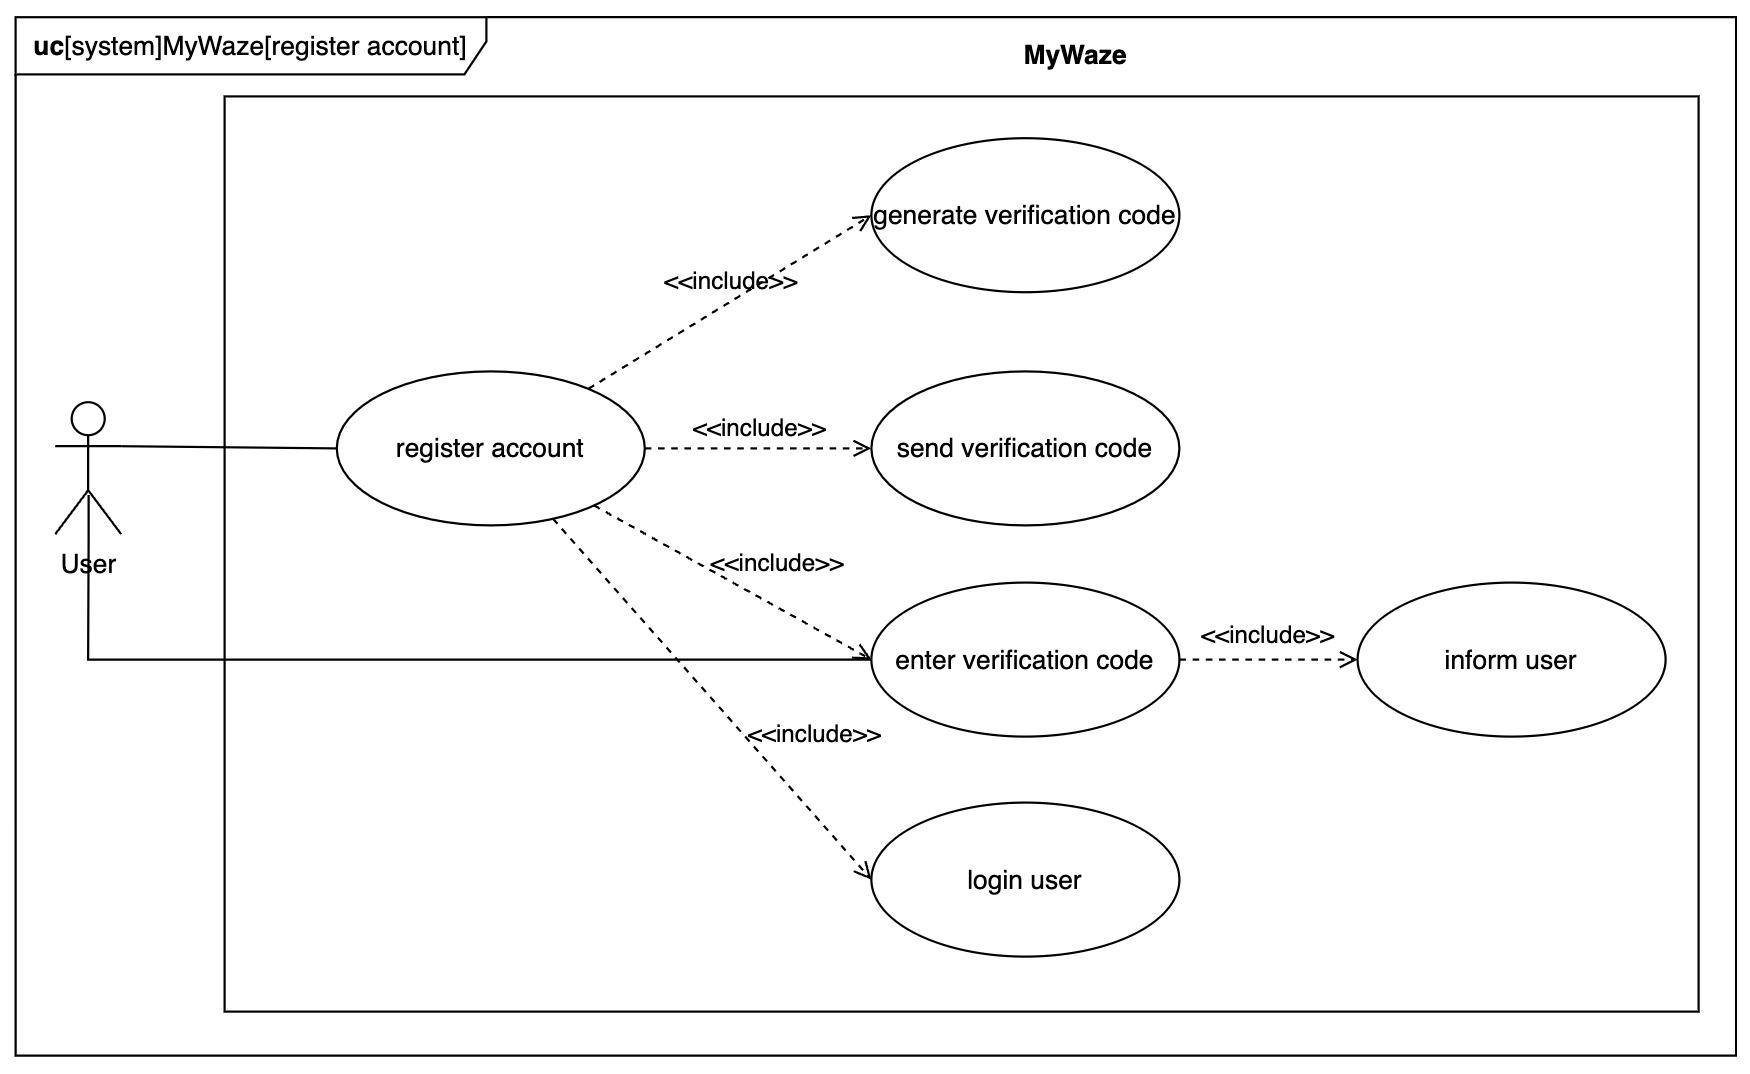
\includegraphics[width=\textwidth]{UseCases/Use_Case_Register_Account.png}
  \caption{Use Case Diagram: Register Account}
  \label{fig:useCaseRegisterAccount}
\end{figure}

\begin{figure}[H]
  \centering
  \includegraphics[width=\textwidth]{UseCases/Use_Case_Shared_Ride.png}
  \caption{Use Case Diagram: Shared Ride}
  \label{fig:useCaseSharedRide}
\end{figure}

\begin{figure}[H]
  \centering
  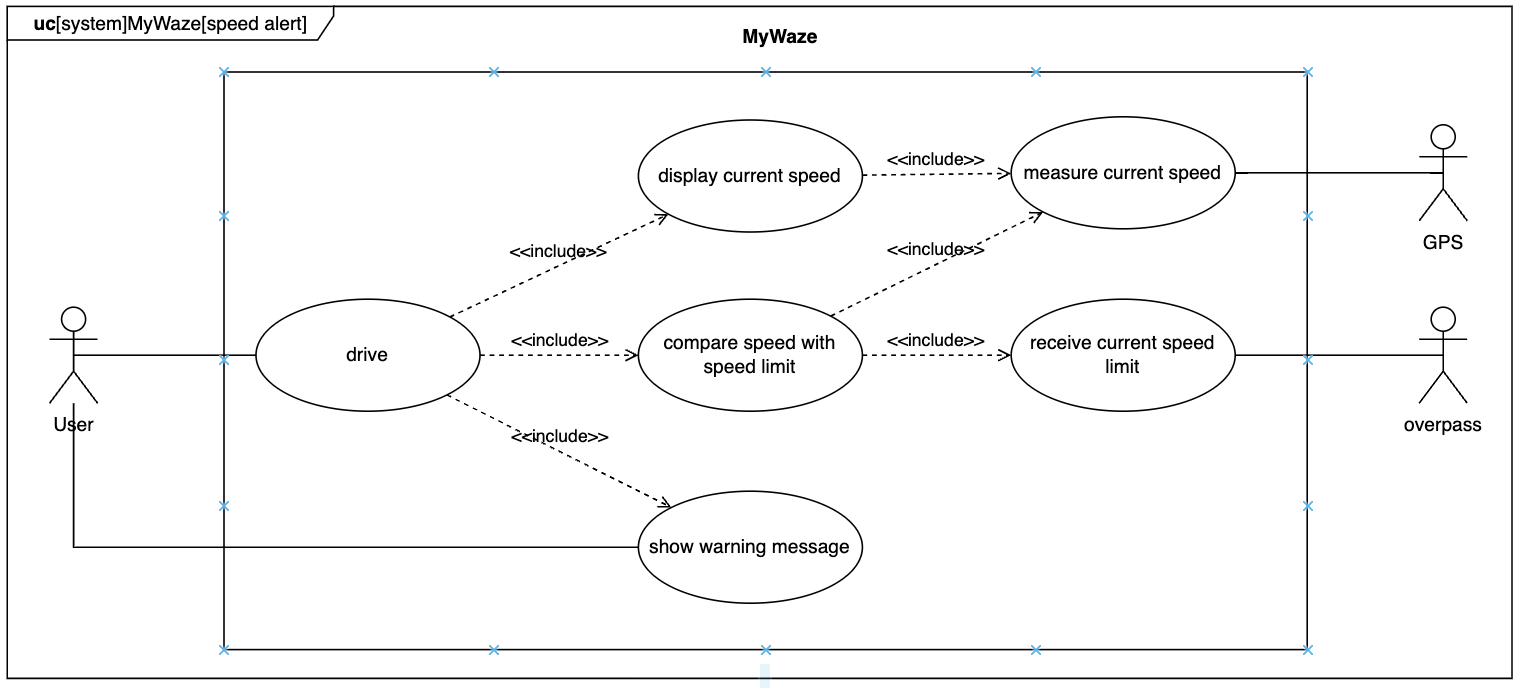
\includegraphics[width=\textwidth]{UseCases/Use_Case_Speed_Alert.png}
  \caption{Use Case Diagram: Speed Alert}
  \label{fig:useCaseSpeedAlert}
\end{figure}

\begin{figure}[H]
  \centering
  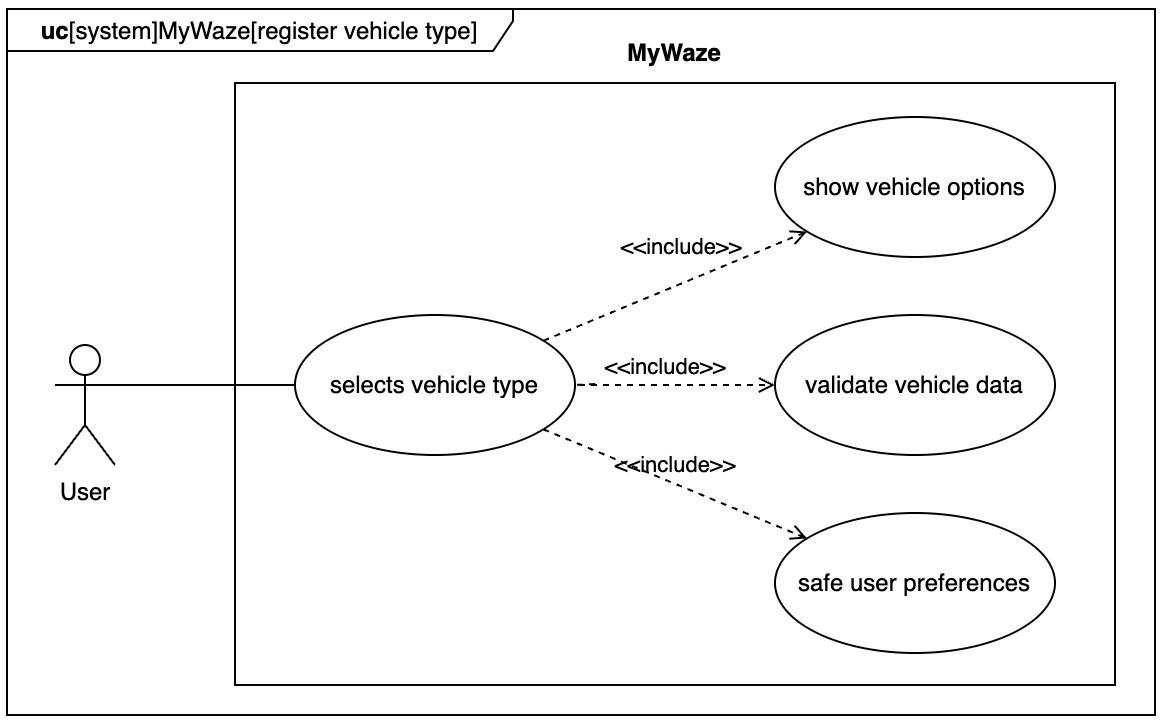
\includegraphics[width=\textwidth]{UseCases/Use_Case_Vehicle_Type.png}
  \caption{Use Case Diagram: Register Vehicle Type}
  \label{fig:useCaseVehicleType}
\end{figure}

\section*{Logical View}
\subsection*{System Decomposition}
\begin{figure}[H]
  \centering
  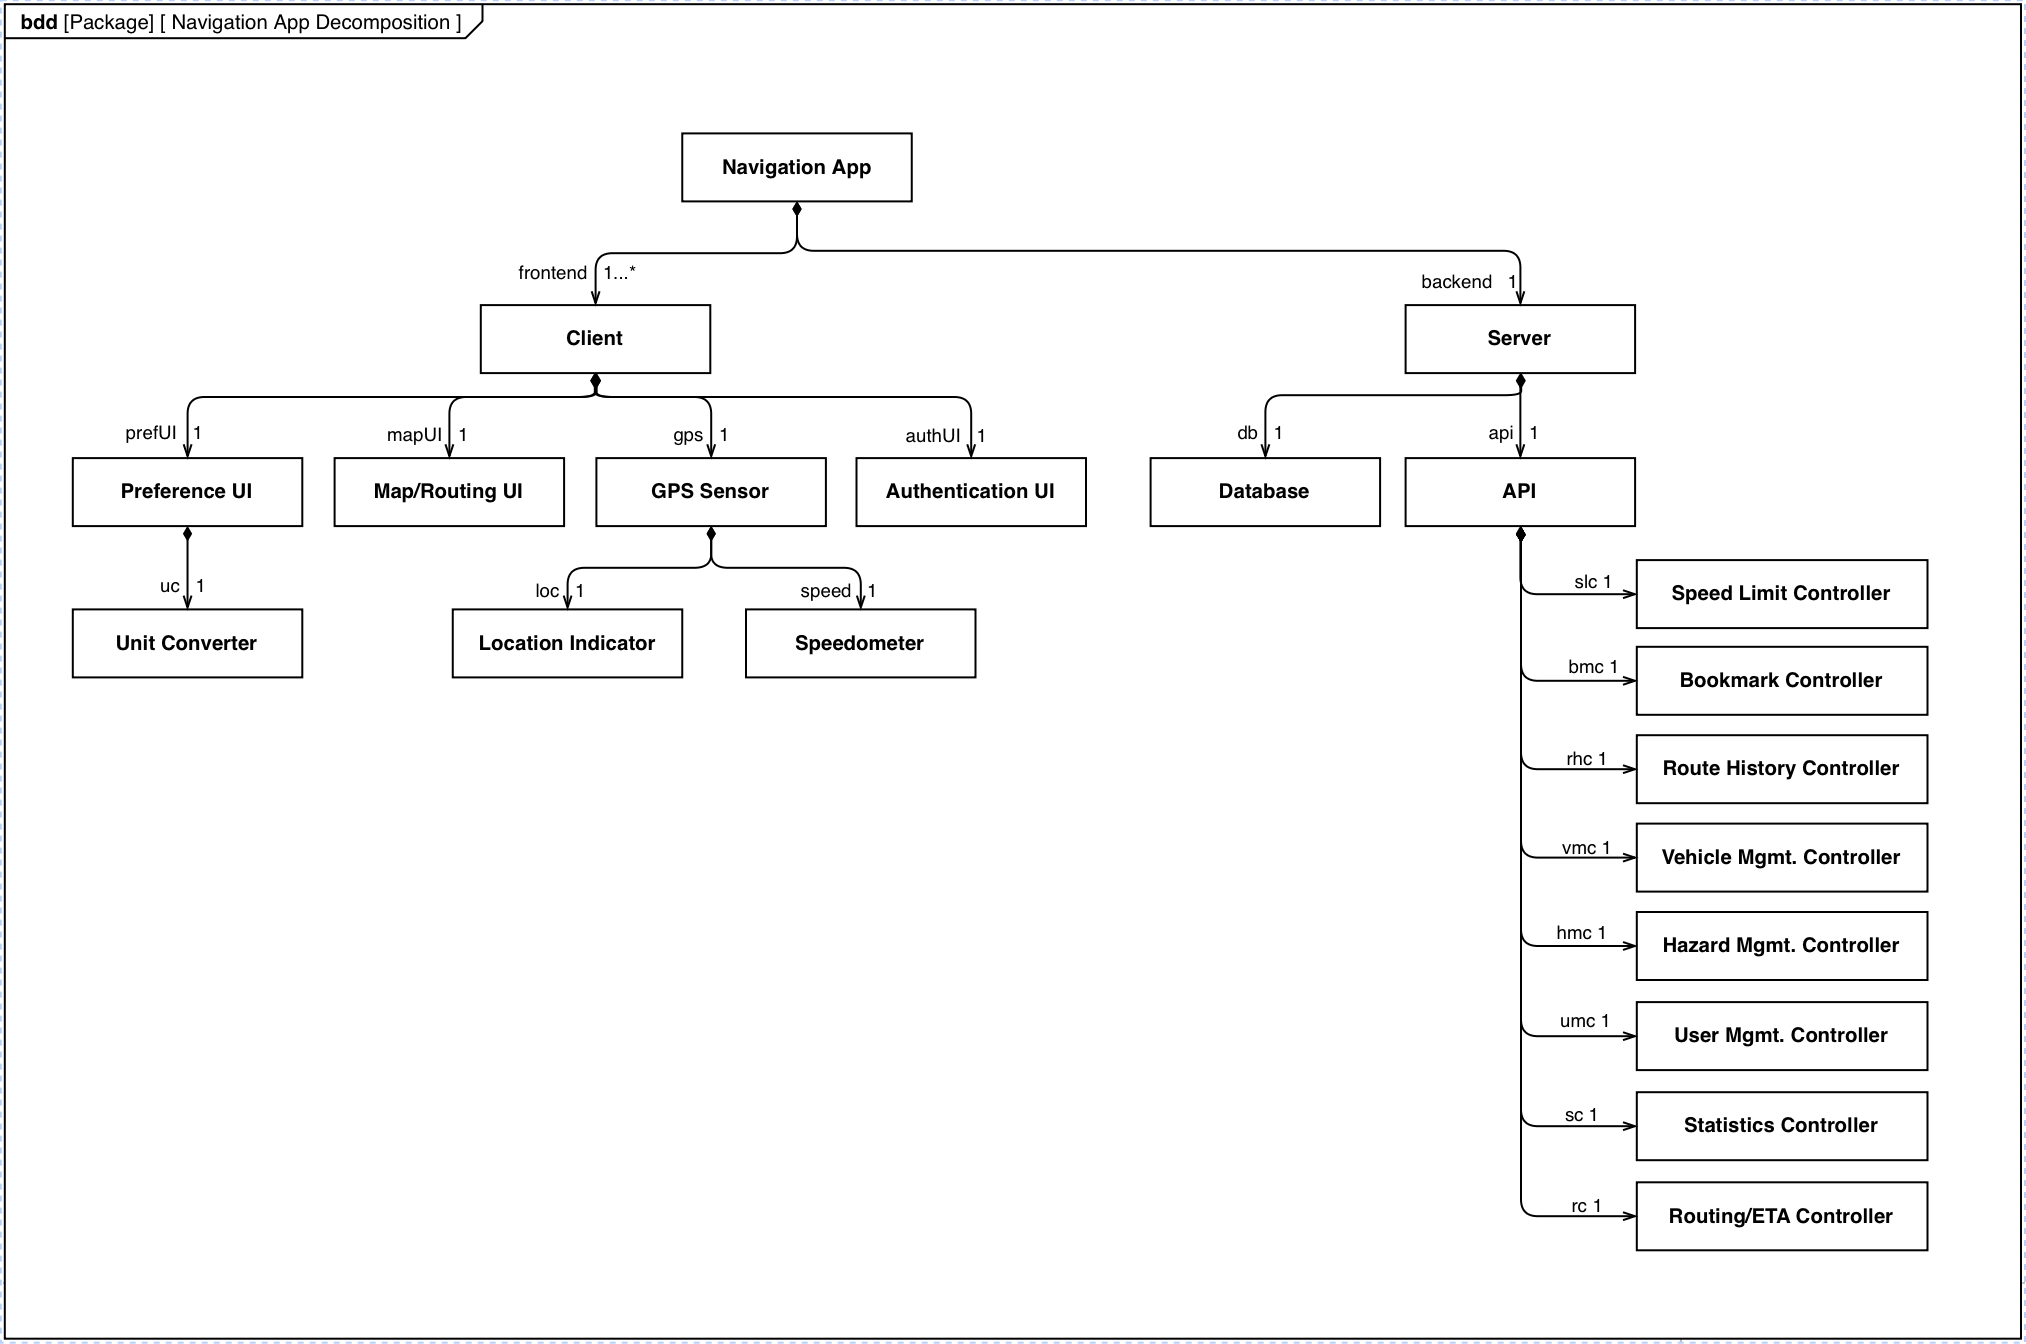
\includegraphics[width=\textwidth]{images/logicalView.png}
  \caption{MyWaze Decomposition}
  \label{fig:Decomposition}
\end{figure}

\subsection*{Navigation Domain}

\begin{figure}[H]
  \centering
  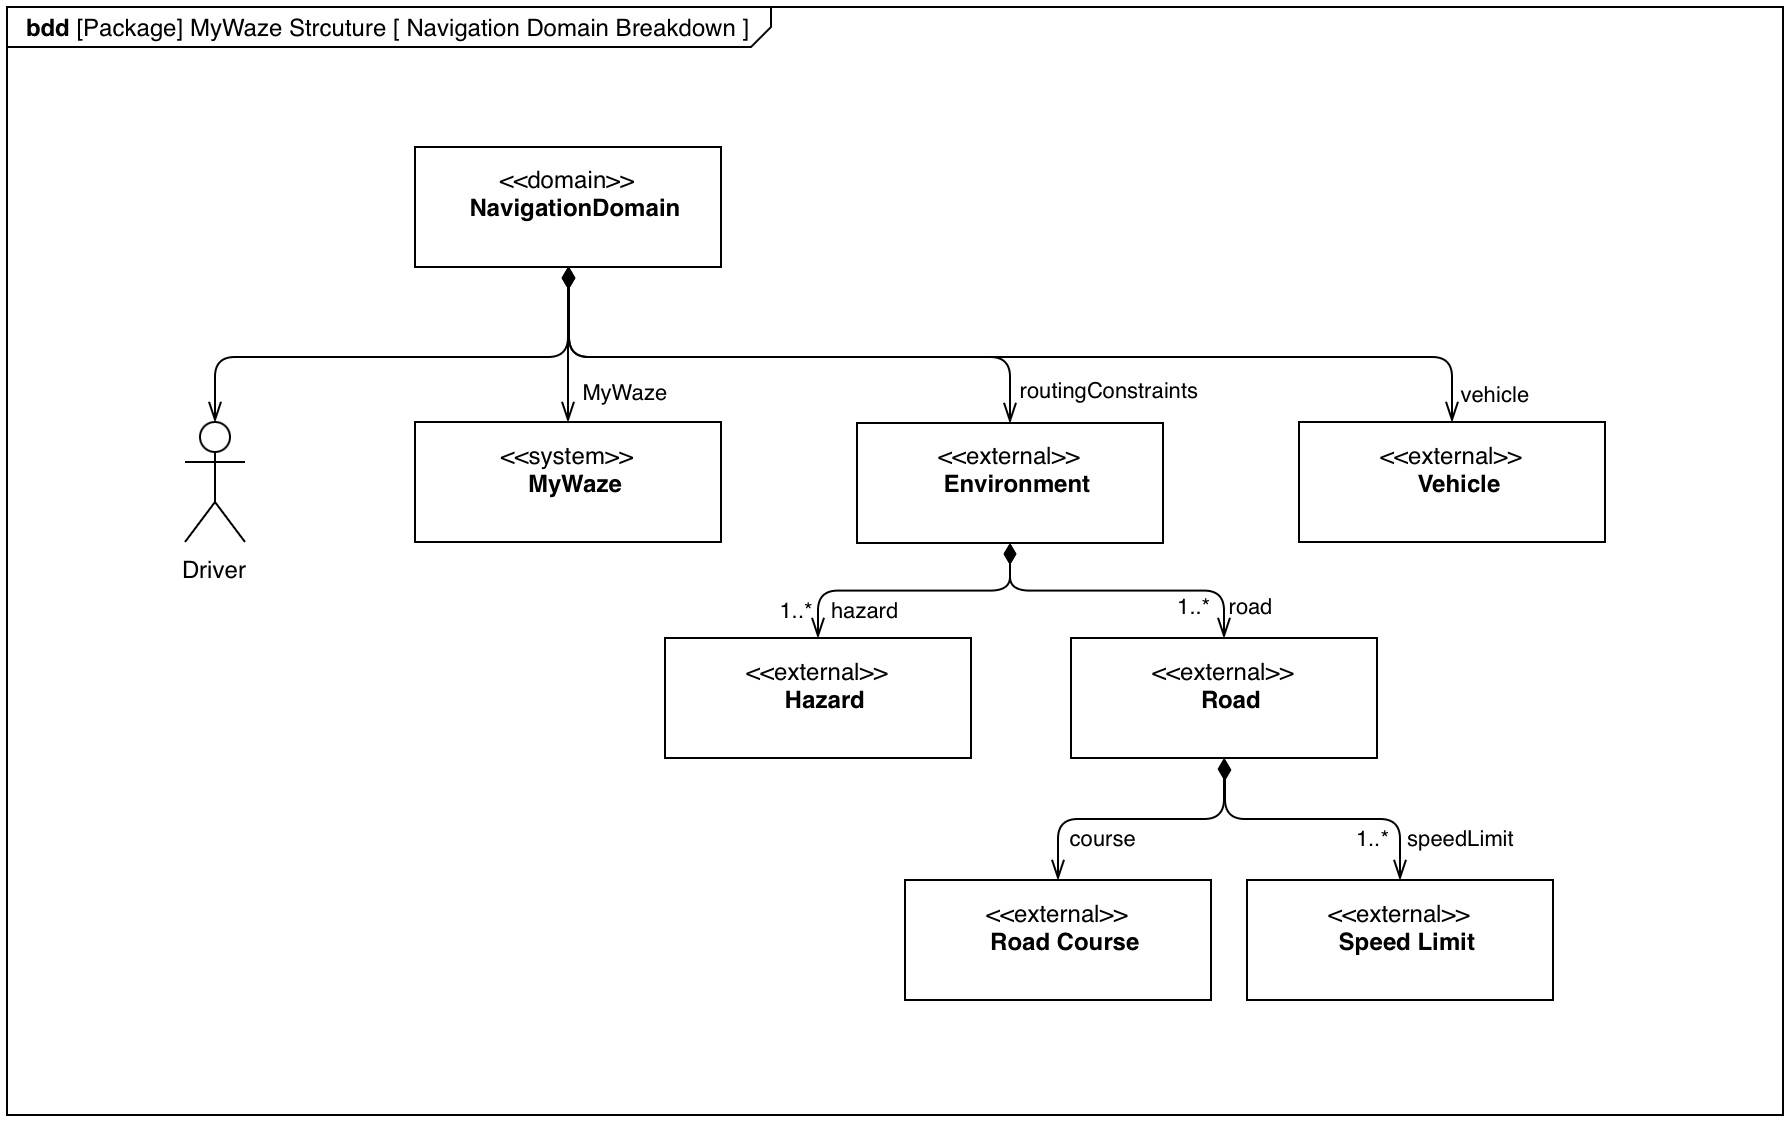
\includegraphics[width=\textwidth]{images/domain.png}
  \caption{Navigation Domain}
  \label{fig:domain}
\end{figure}

\section*{Process View}

\begin{figure}[H]
  \centering
  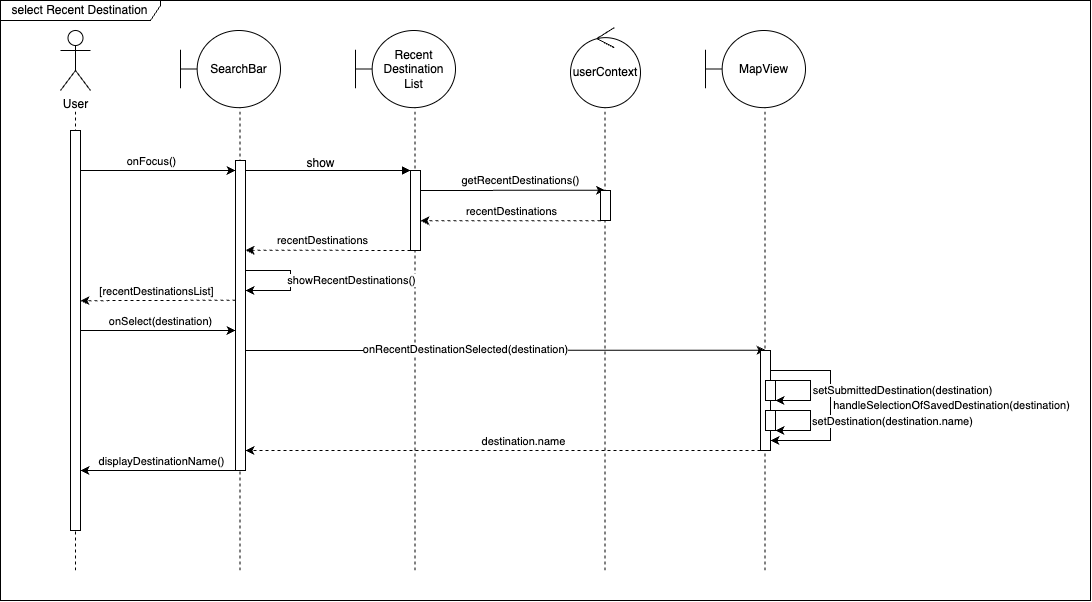
\includegraphics[width=\textwidth]{images/sequence_diagramm/recentDestinations_squenceDiagramm-Page.drawio.png}
  \caption{Sequence Diagram: Recent Destinations}
  \label{fig:sequence_recents}
\end{figure}

\begin{figure}[H]
  \centering
  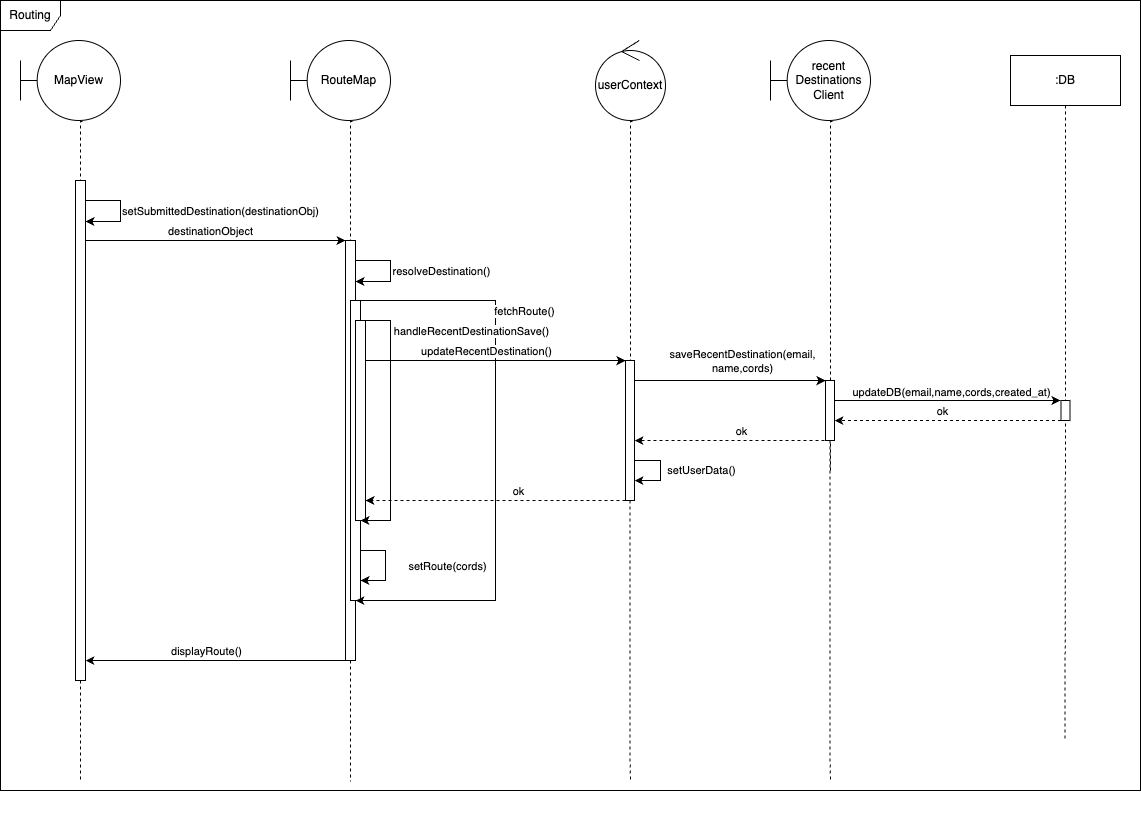
\includegraphics[width=\textwidth]{images/sequence_diagramm/routing_squenceDiagramm-Seite.drawio.png}
  \caption{Sequence Diagram: Routing}
  \label{fig:sequence_routing}
\end{figure}

\begin{figure}[H]
  \centering
  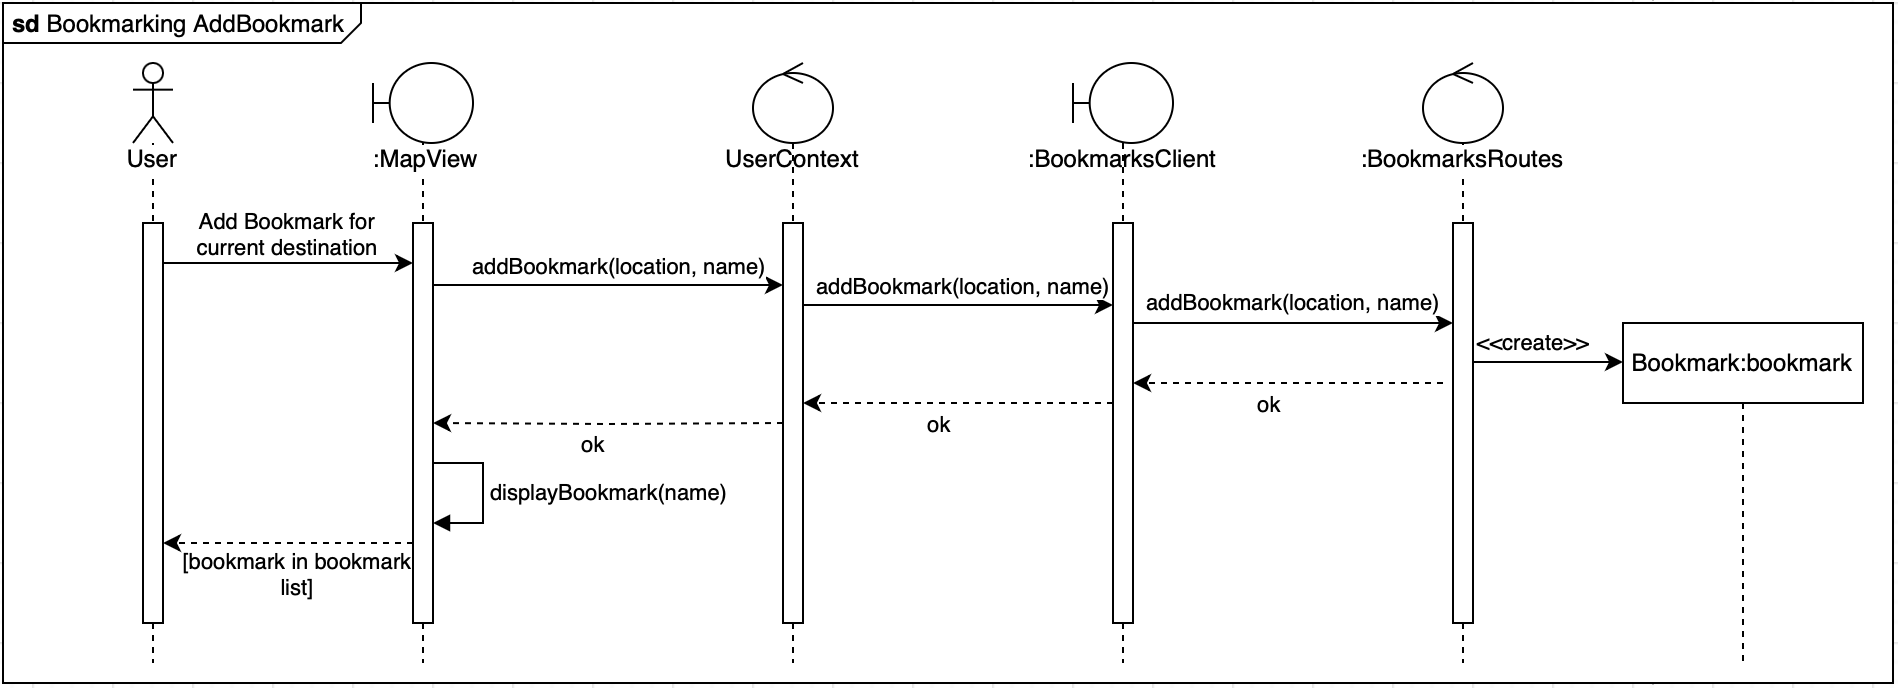
\includegraphics[width=\textwidth]{images/sequence_diagramm/bookmarking_addBookmark.png}
  \caption{Sequence Diagram: Bookmarking (add)}
  \label{fig:sequence_bookmarks}
\end{figure}

\begin{figure}[H]
  \centering
  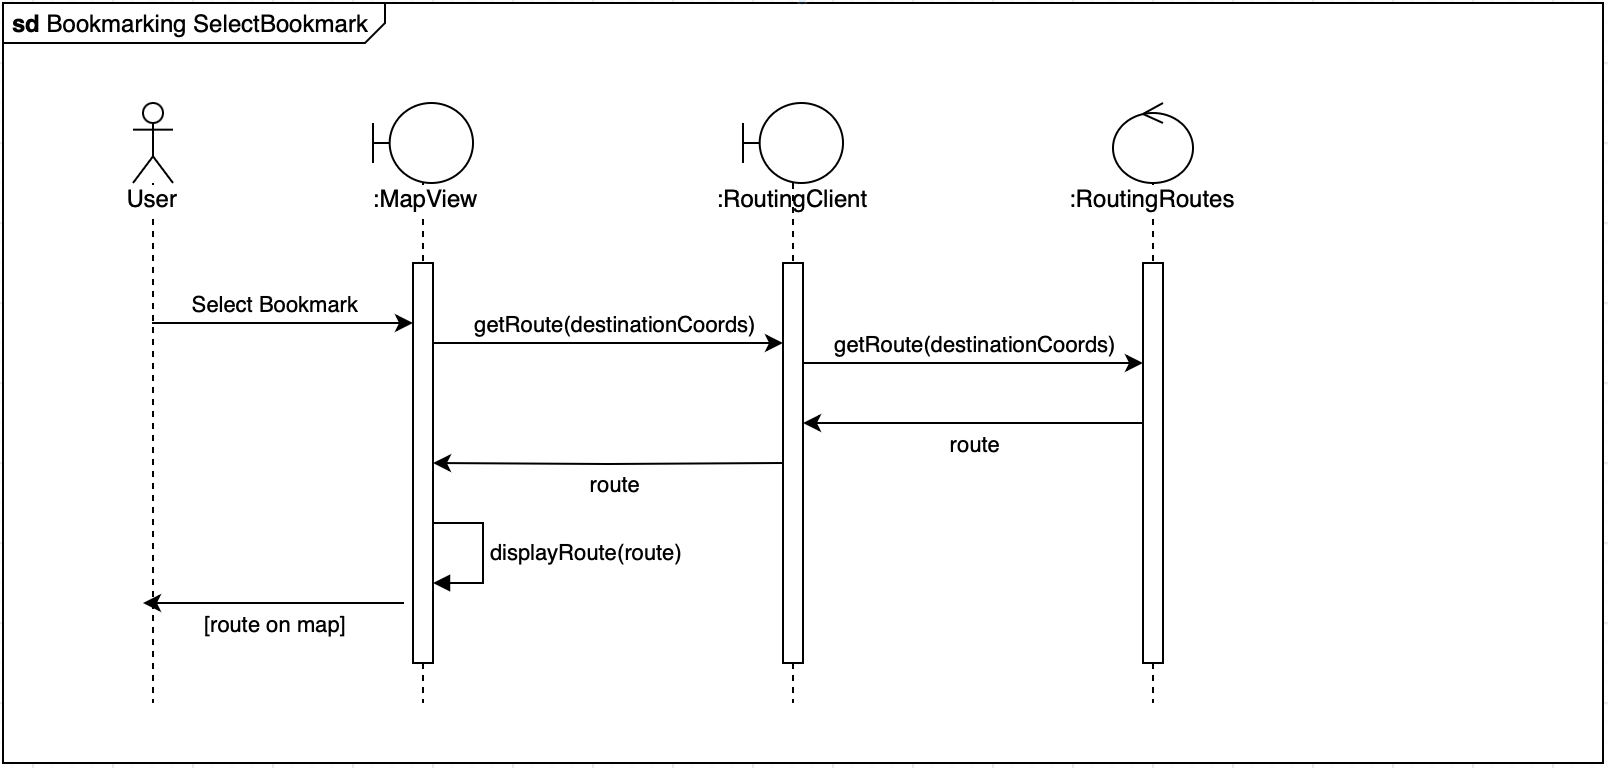
\includegraphics[width=\textwidth]{images/sequence_diagramm/bookmarking_selectBookmark.png}
  \caption{Sequence Diagram: Bookmarking (select)}
  \label{fig:sequence_bookmarks1}
\end{figure}

\begin{figure}[H]
  \centering
  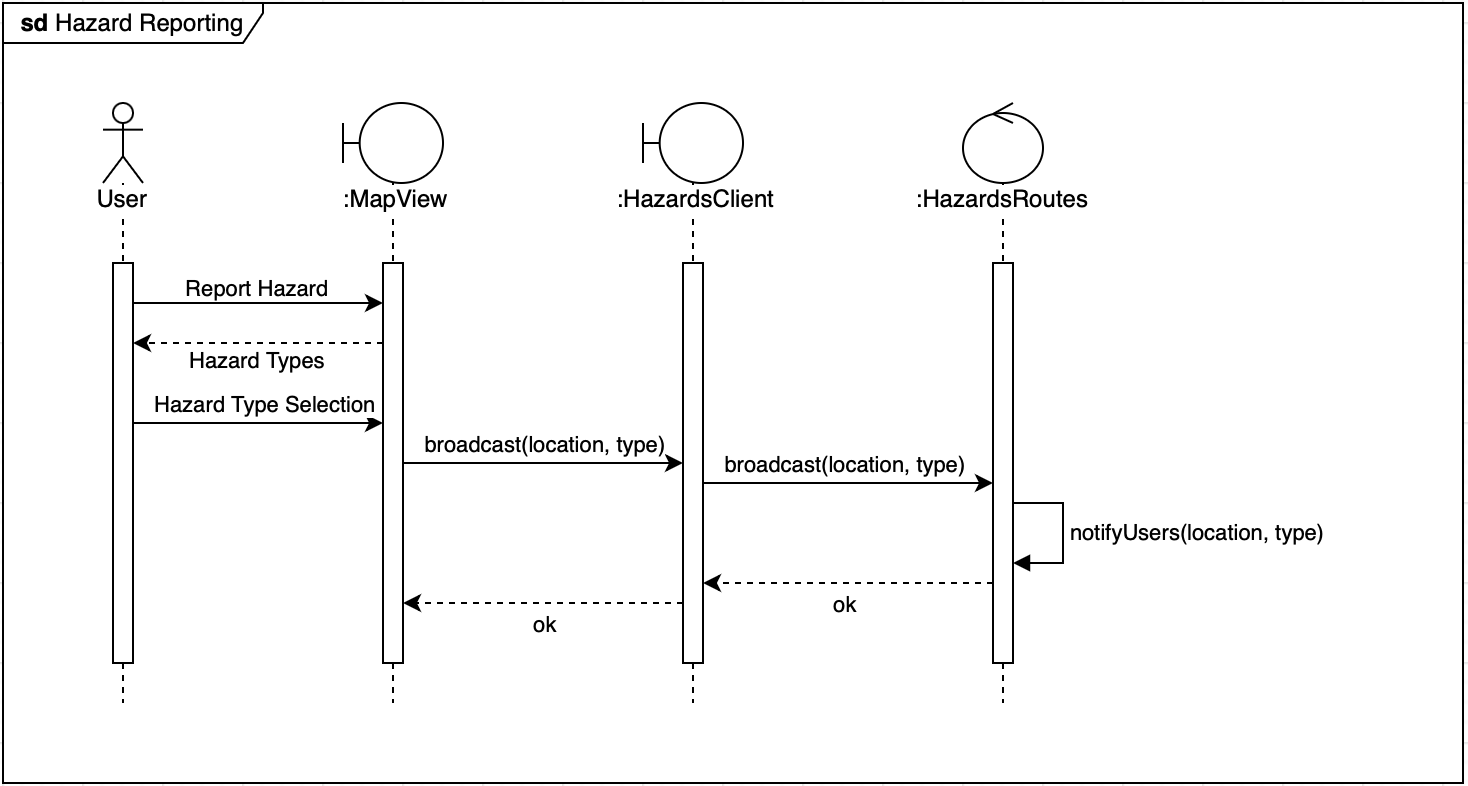
\includegraphics[width=\textwidth]{images/sequence_diagramm/hazards_report.png}
  \caption{Sequence Diagram: Hazards (report)}
  \label{fig:sequence_bookmarks}
\end{figure}

\begin{figure}[H]
  \centering
  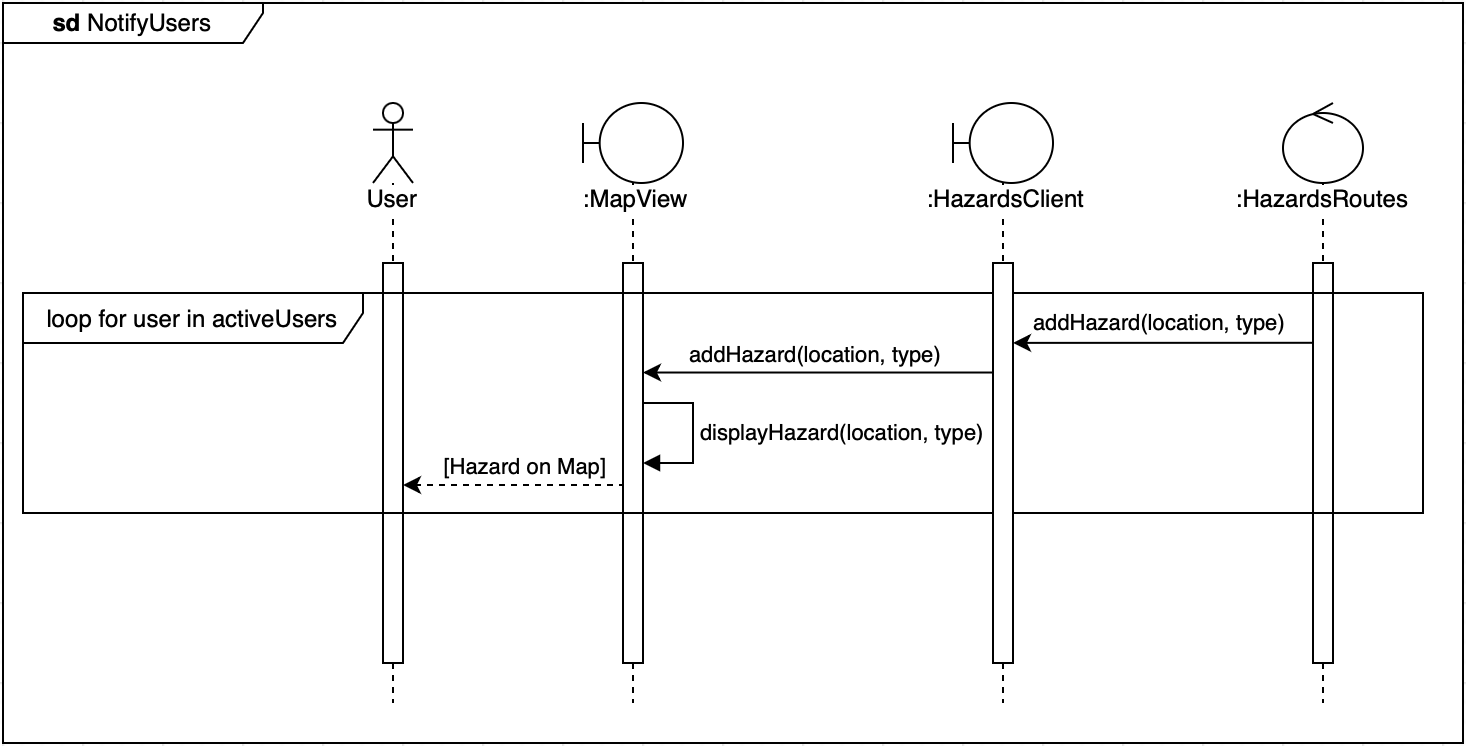
\includegraphics[width=\textwidth]{images/sequence_diagramm/hazards_notify.png}
  \caption{Sequence Diagram: Hazards (notify)}
  \label{fig:sequence_bookmarks1}
\end{figure}

\begin{figure}[H]
  \centering
  \includegraphics[width=\textwidth]{images/sequence_diagramm/loadUserData_sequenceDiagramm.drawio.png}
  \caption{Sequence Diagram: User Data}
  \label{fig:sequence_userData}
\end{figure}

\begin{figure}[H]
  \centering
  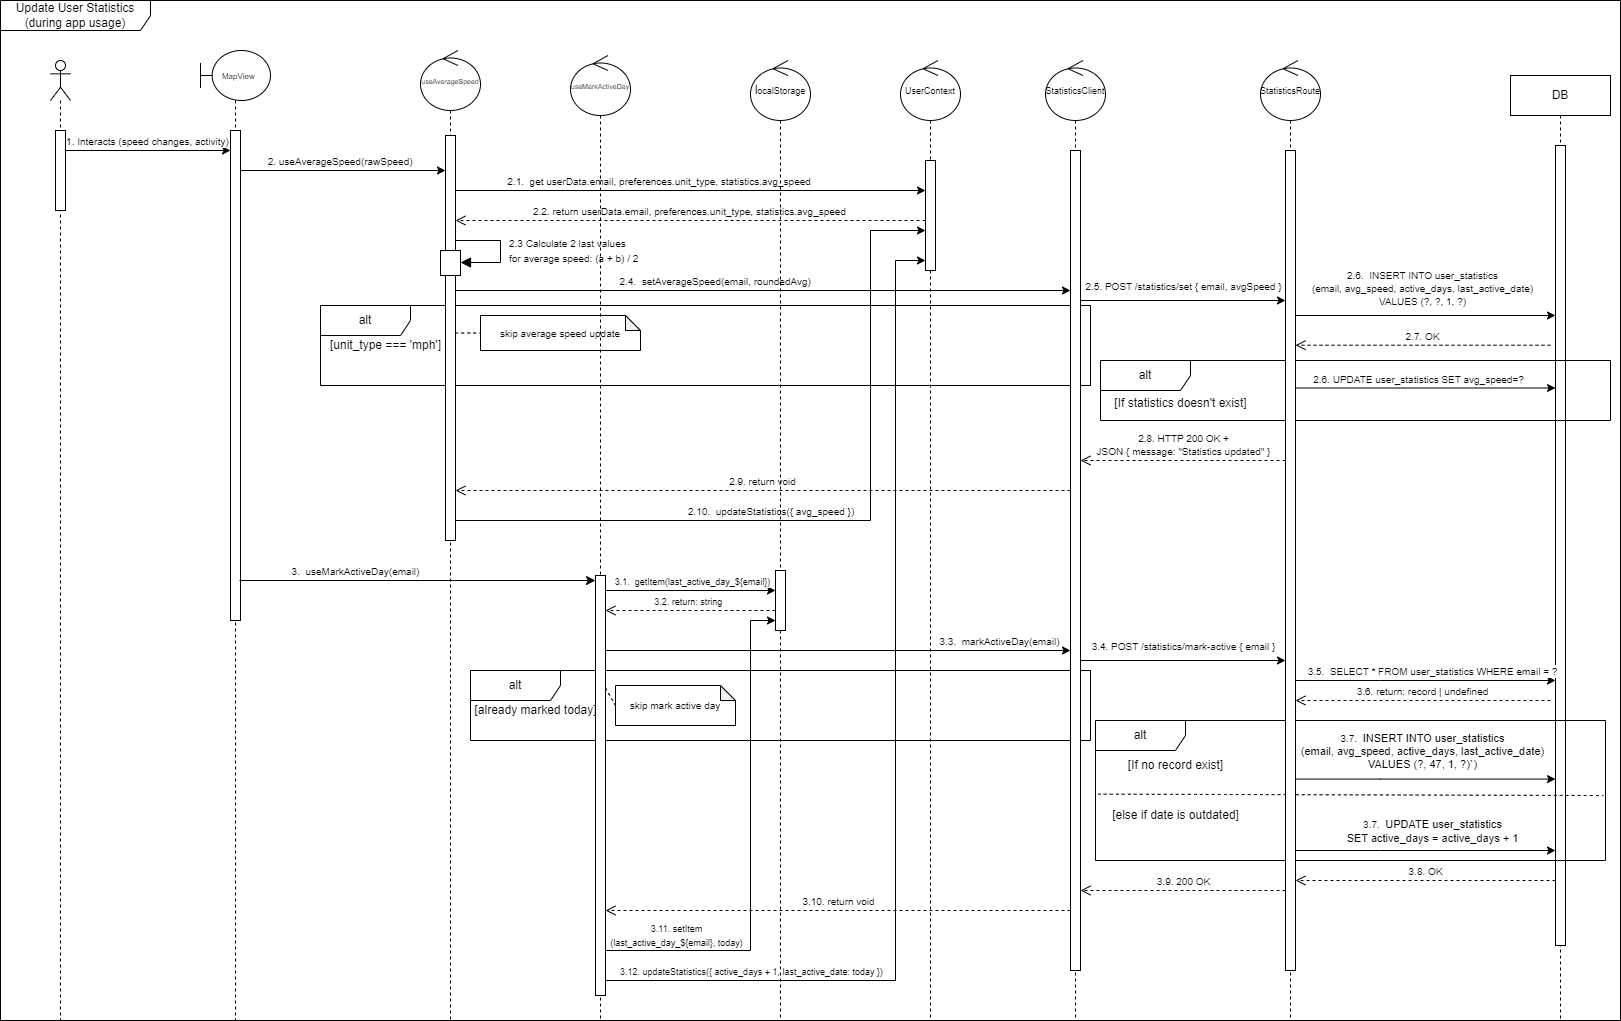
\includegraphics[width=\textwidth]{images/sequence_diagramm/updateUserStatistics_sequenceDiagram.png}
  \caption{Sequence Diagram: Update Statistics}
  \label{fig:sequence_stats}
\end{figure}

\section*{Development View}
\begin{figure}[H]
  \centering
  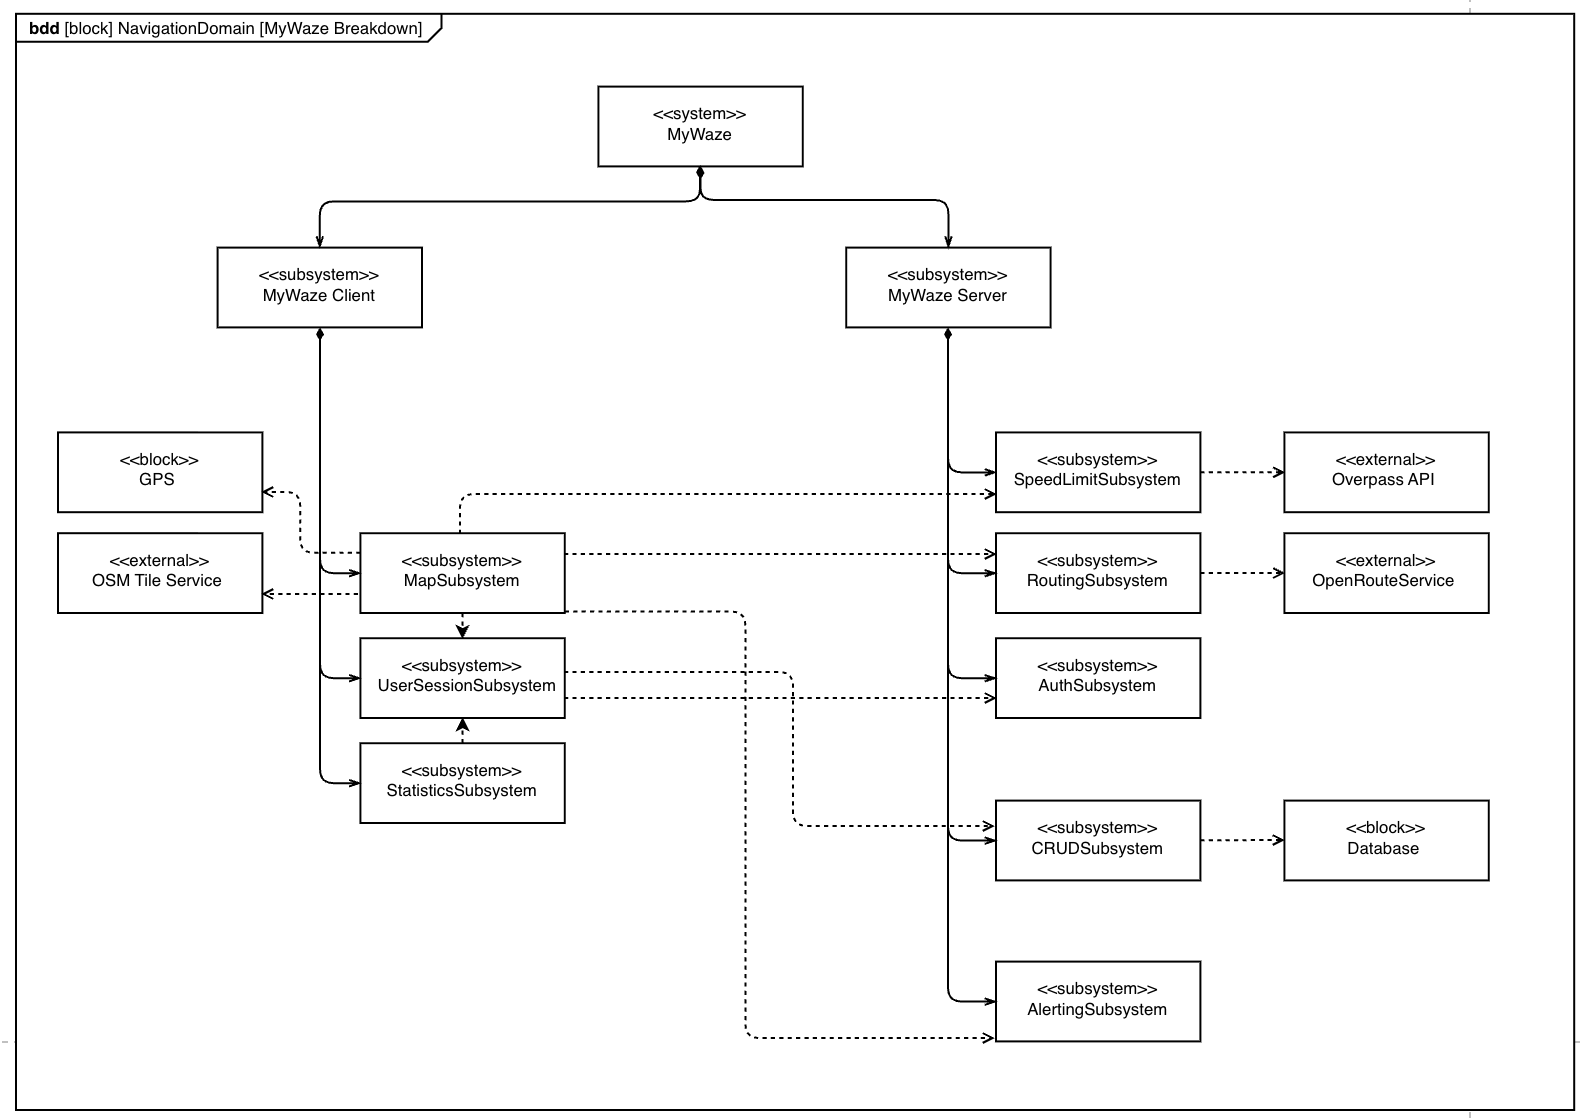
\includegraphics[width=\textwidth]{images/Development_View_Subsystems.png}
  \caption{MyWaze Subsystems}
  \label{fig:subsystems}
\end{figure}

\begin{figure}[H]
  \centering
  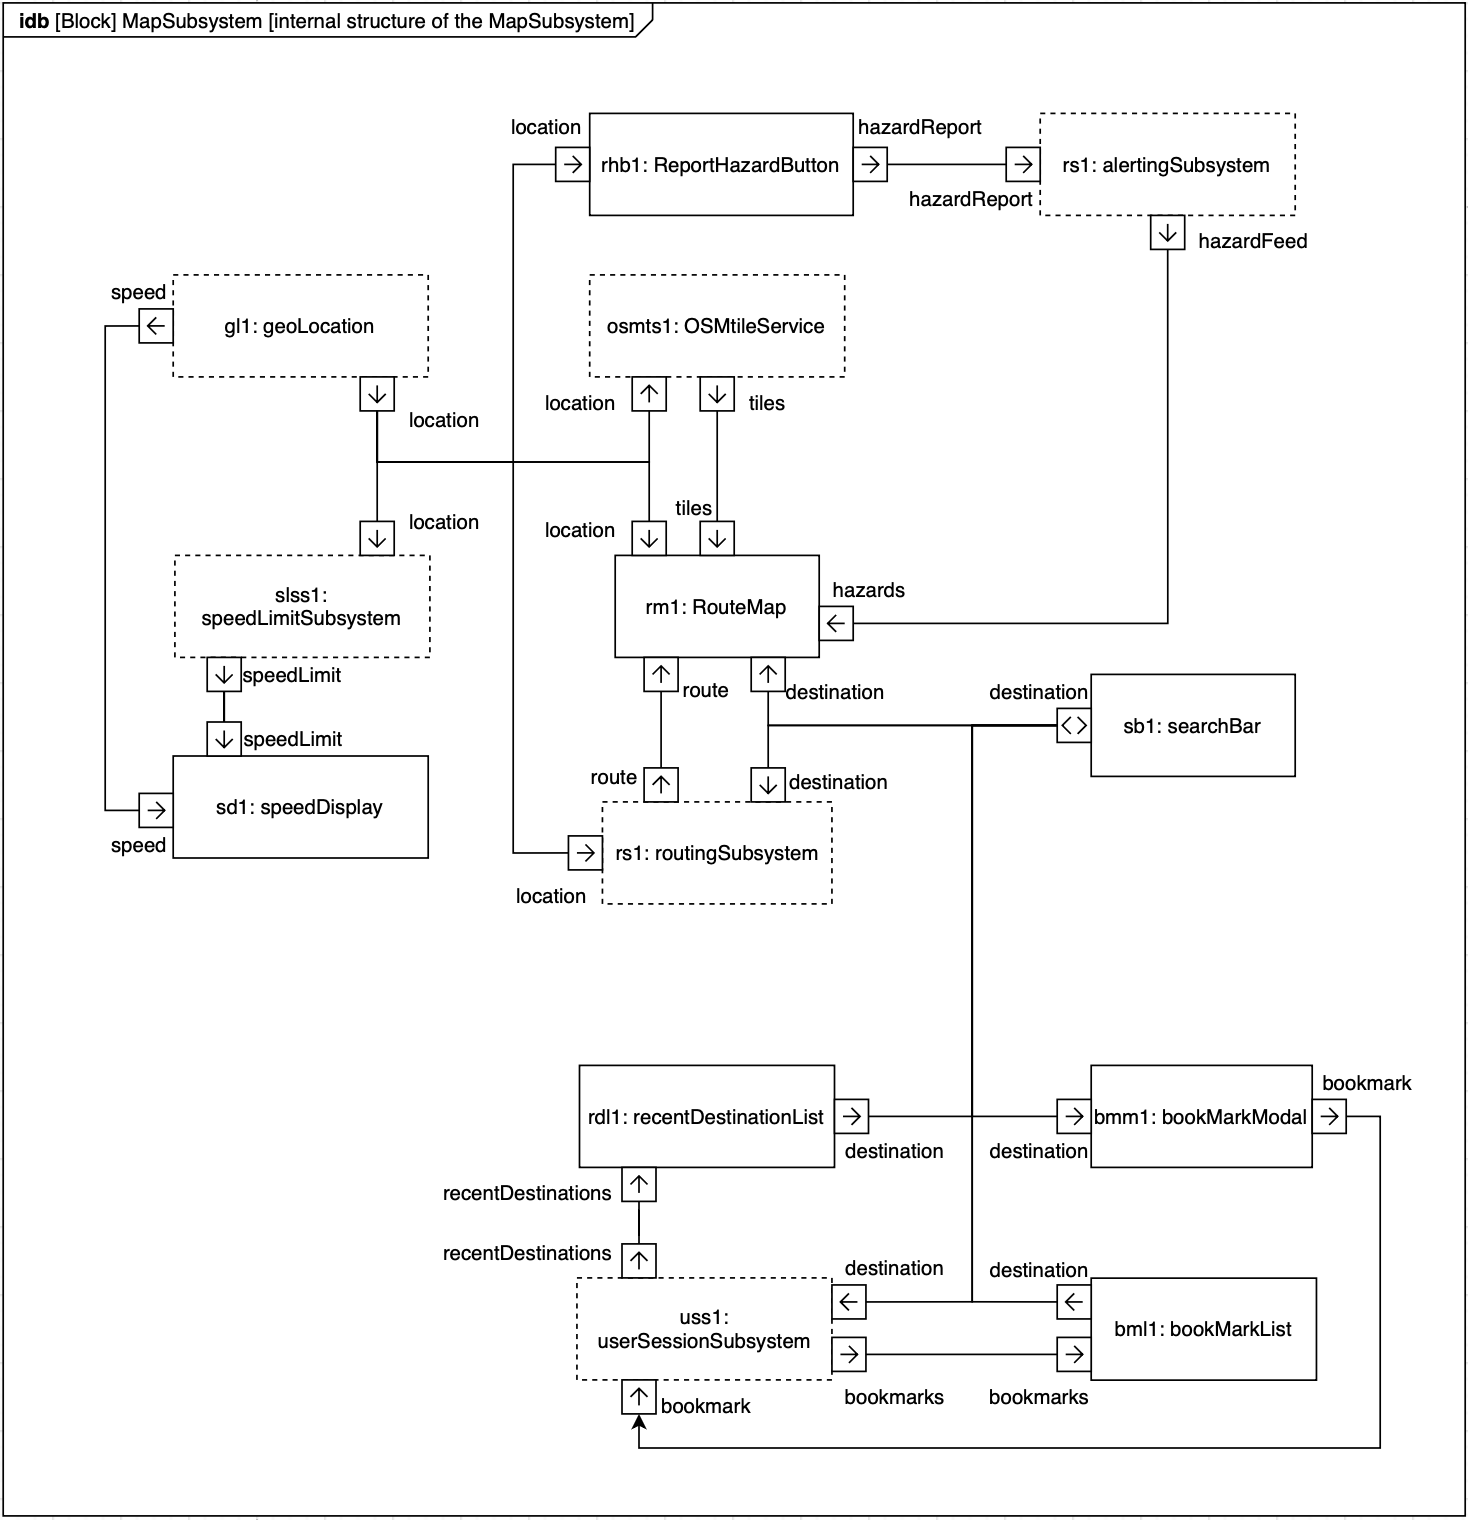
\includegraphics[width=\textwidth]{Internal_Block_Diagrams/IBD_Map.png}
  \caption{Internal Block Diagram: Map Subsystem}
  \label{fig:subsystems_map}
\end{figure}

\begin{figure}[H]
  \centering
  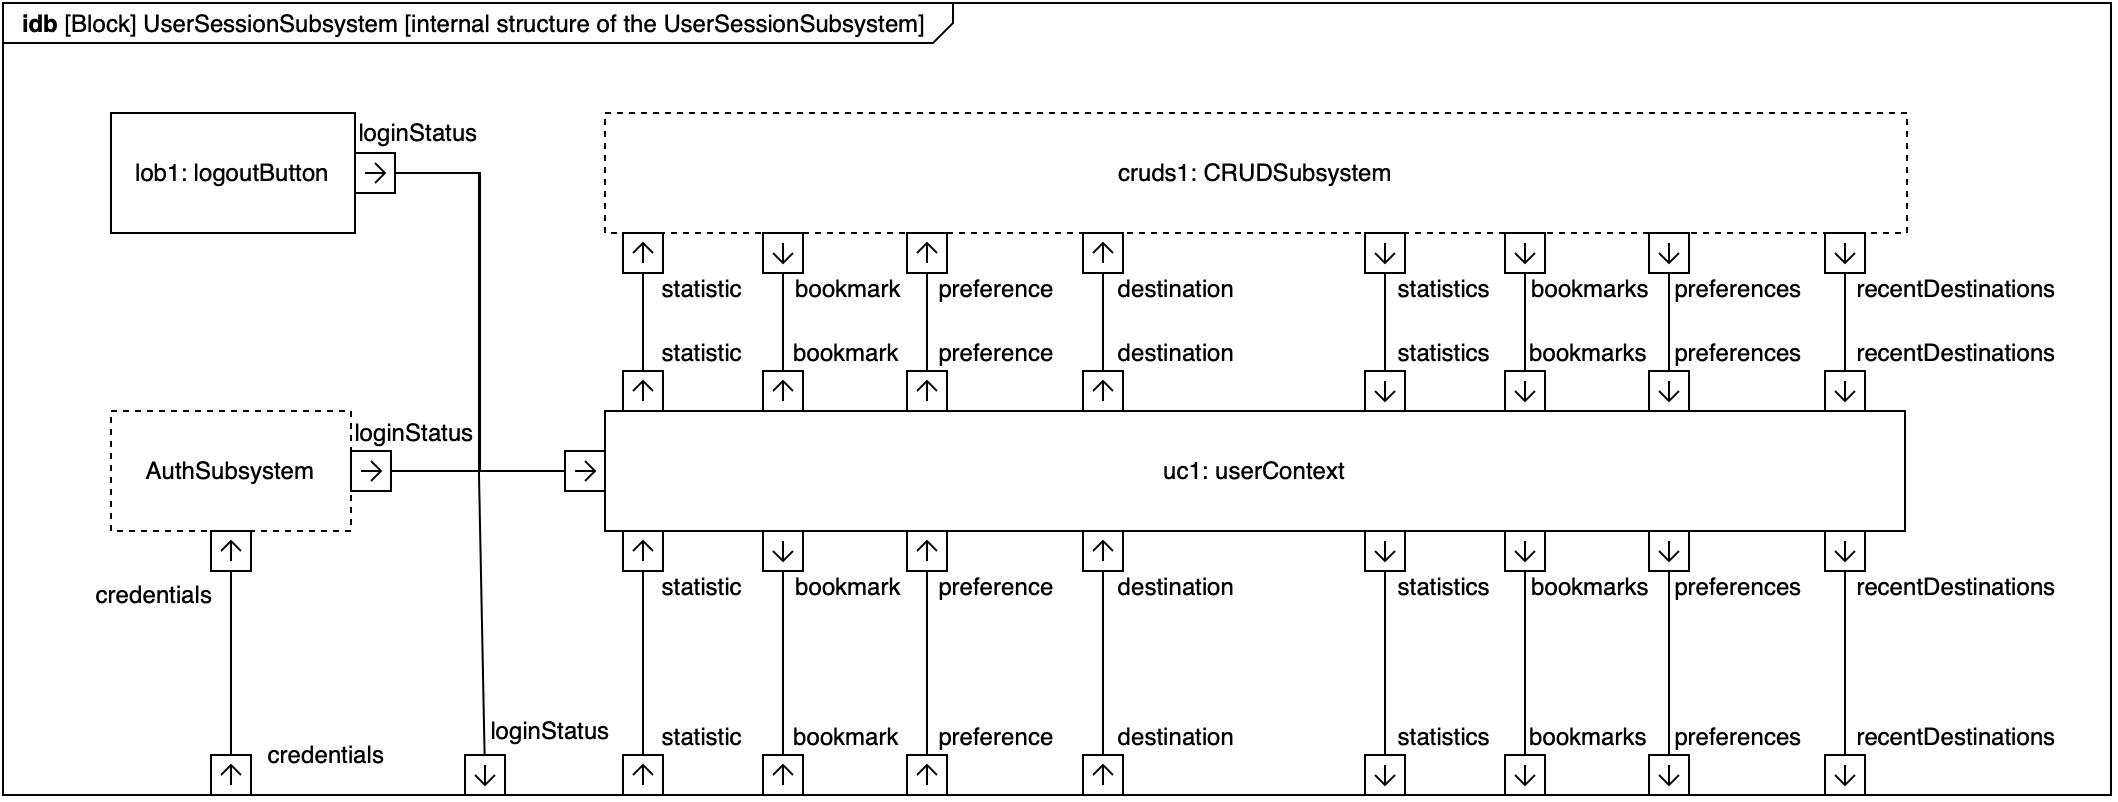
\includegraphics[width=\textwidth]{Internal_Block_Diagrams/IBD_UserSession.png}
  \caption{Internal Block Diagram: UserSession Subsystem}
  \label{fig:subsystems_session}
\end{figure}

\begin{figure}[H]
  \centering
  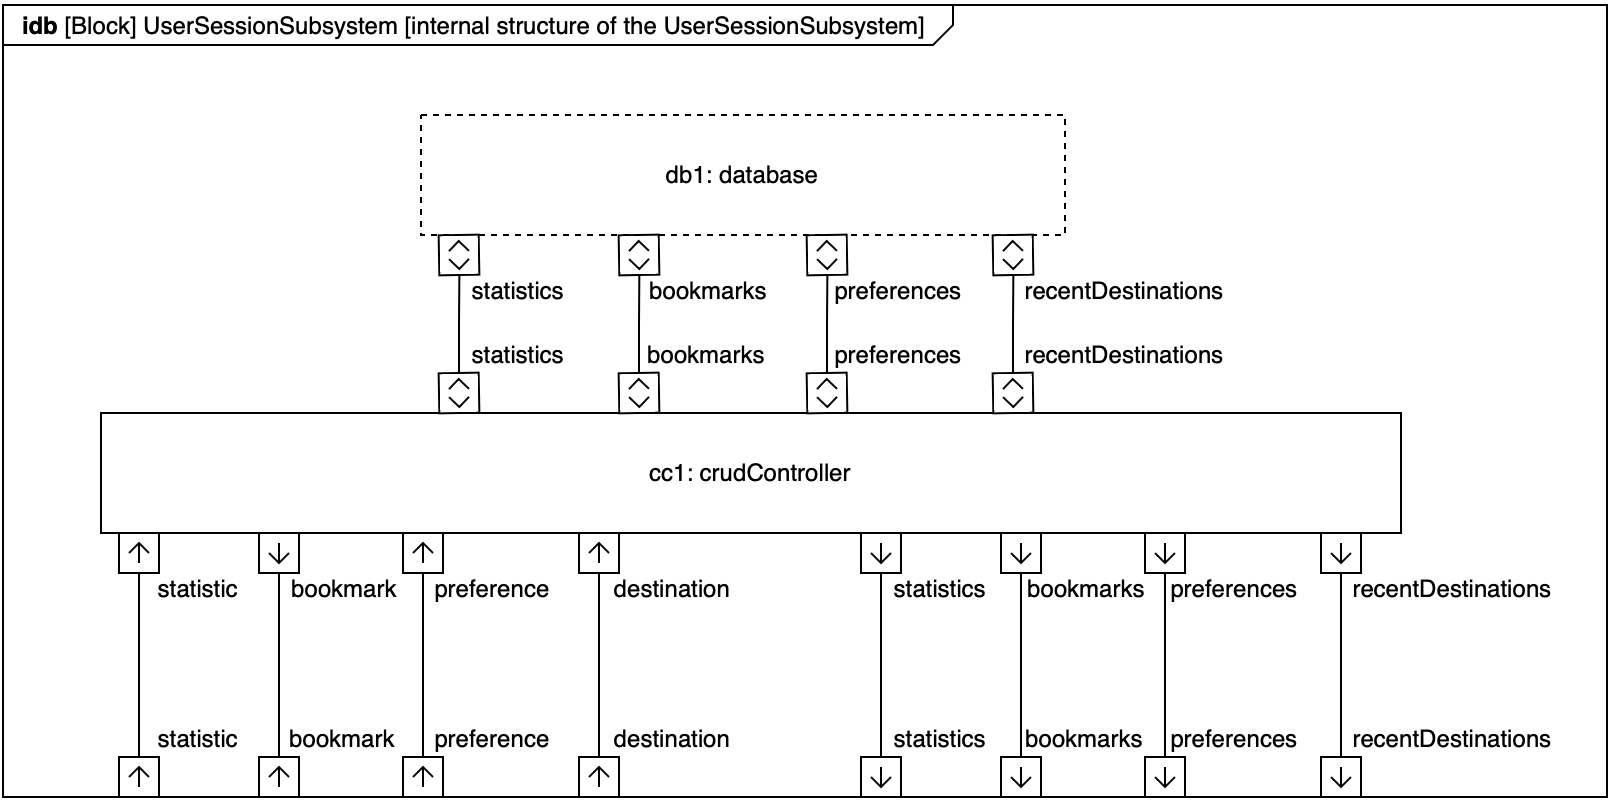
\includegraphics[width=\textwidth]{Internal_Block_Diagrams/IBD_Crud.png}
  \caption{Internal Block Diagram: CRUD Subsystem}
  \label{fig:subsystems_crud}
\end{figure}

\begin{figure}[H]
  \centering
  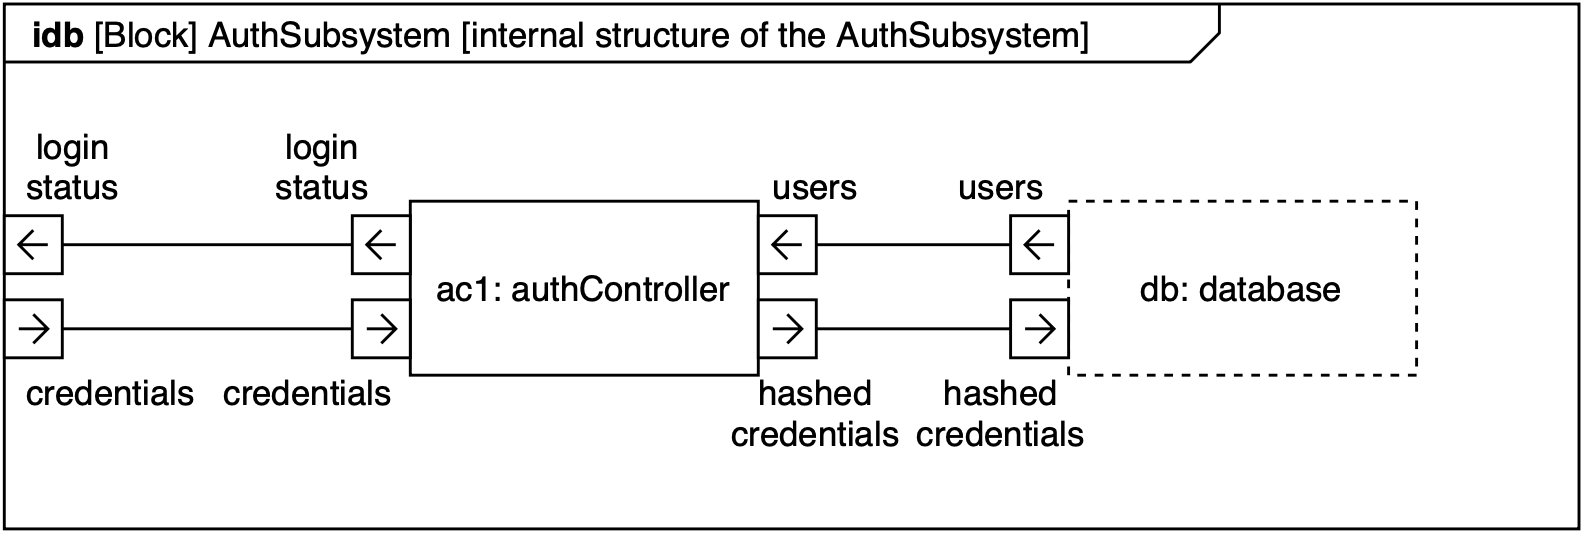
\includegraphics[width=\textwidth]{Internal_Block_Diagrams/IBD_Auth.png}
  \caption{Internal Block Diagram: Auth Subsystem}
  \label{fig:subsystems_auth}
\end{figure}

\begin{figure}[H]
  \centering
  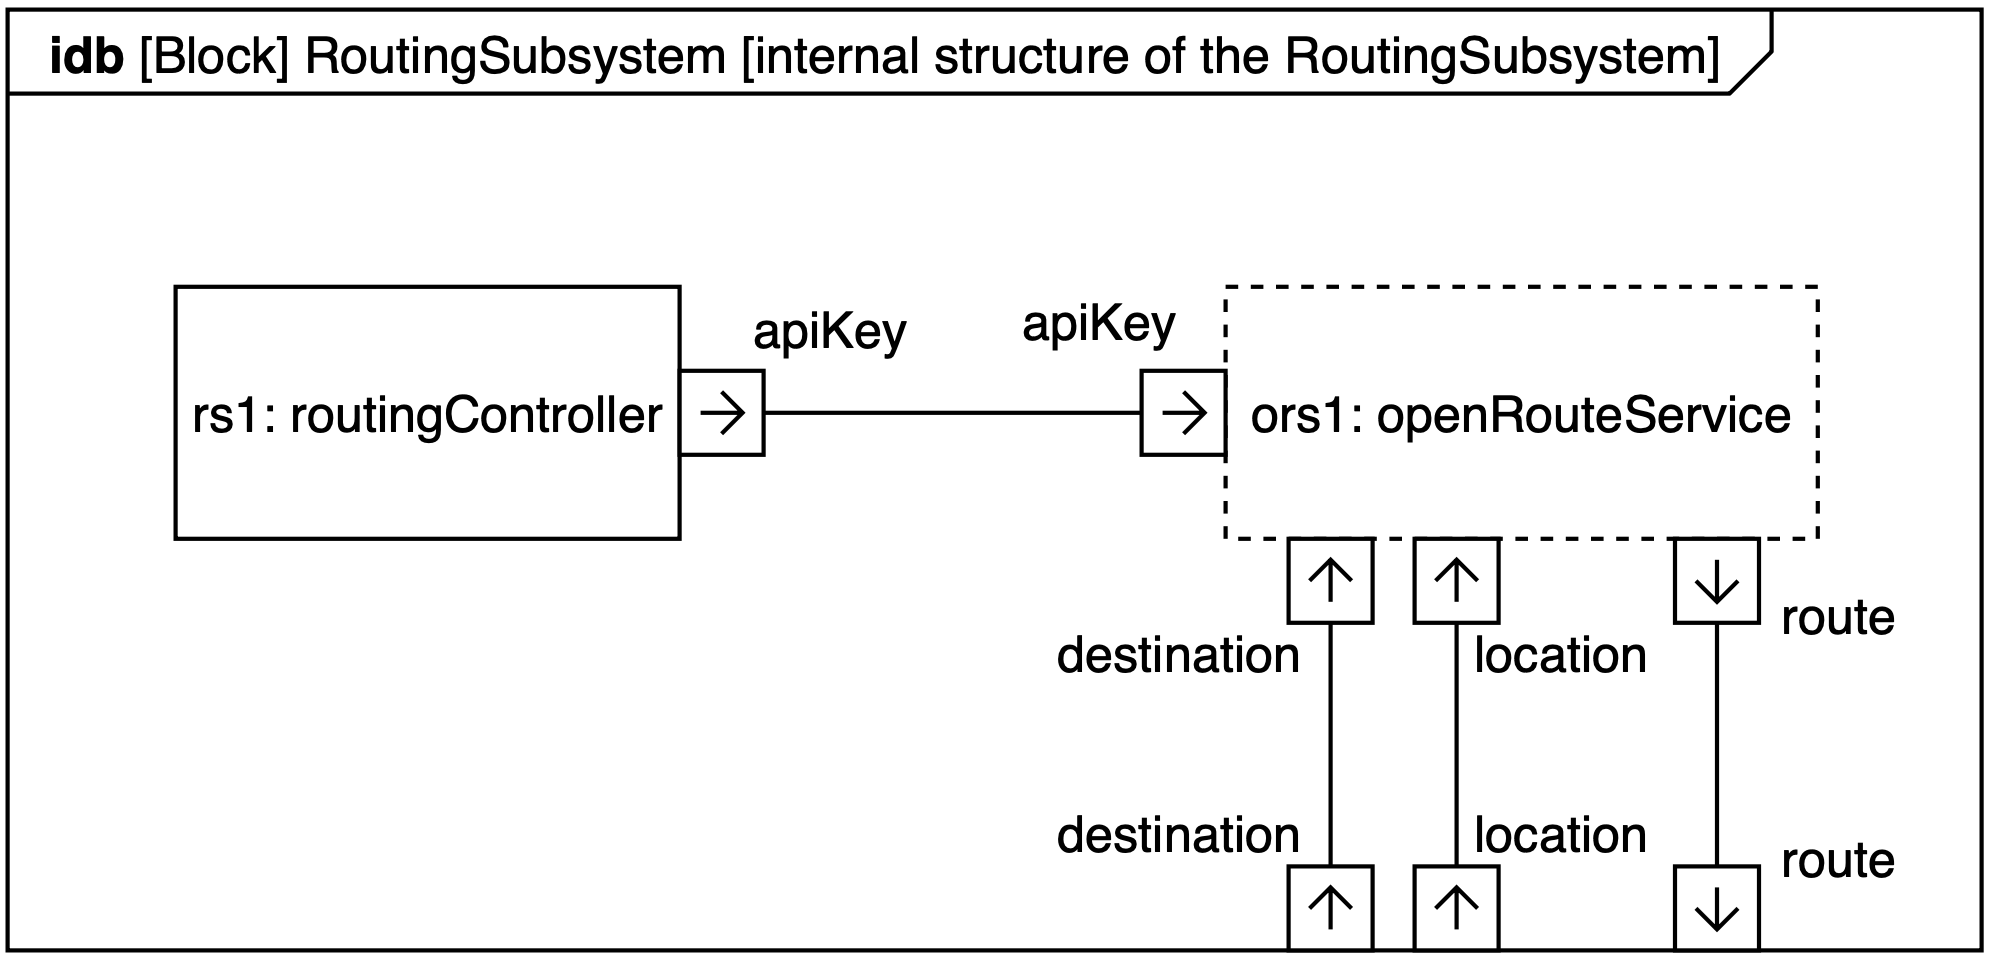
\includegraphics[width=\textwidth]{Internal_Block_Diagrams/IBD_Routing.png}
  \caption{Internal Block Diagram: Routing Subsystem}
  \label{fig:subsystems_routing}
\end{figure}

\begin{figure}[H]
  \centering
  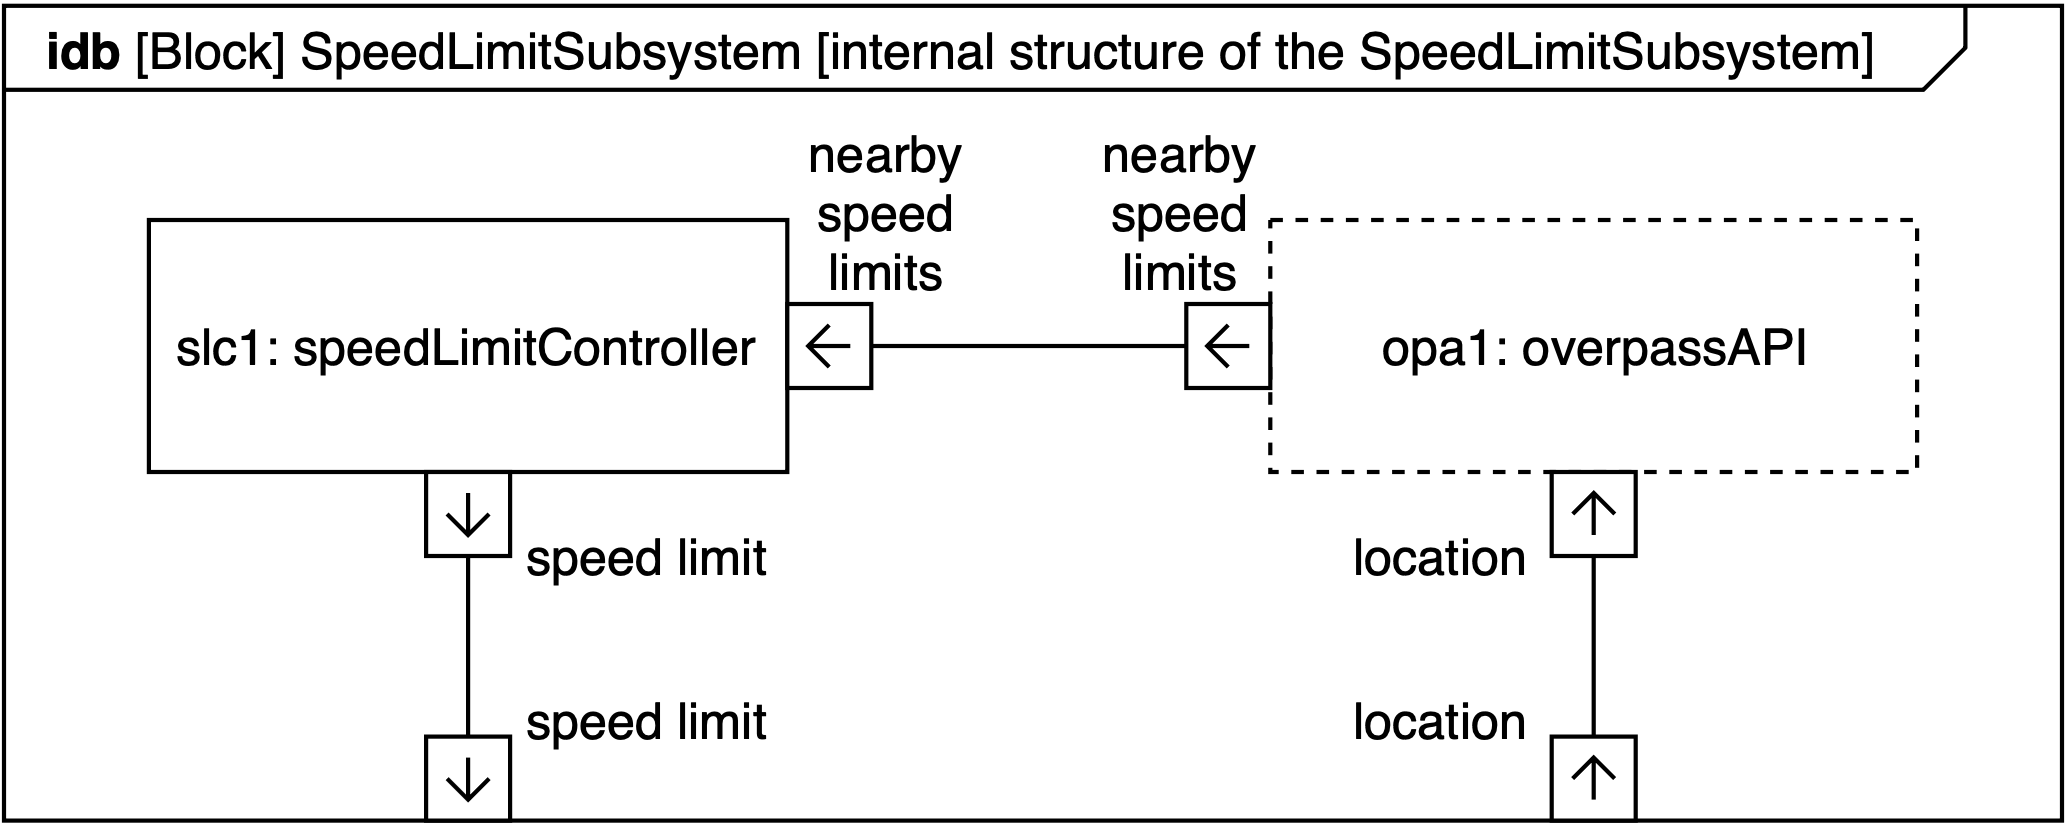
\includegraphics[width=\textwidth]{Internal_Block_Diagrams/IBD_SpeedLimit.png}
  \caption{Internal Block Diagram: Speed Limit Subsystem}
  \label{fig:subsystems_speedlimit}
\end{figure}

\begin{figure}[H]
  \centering
  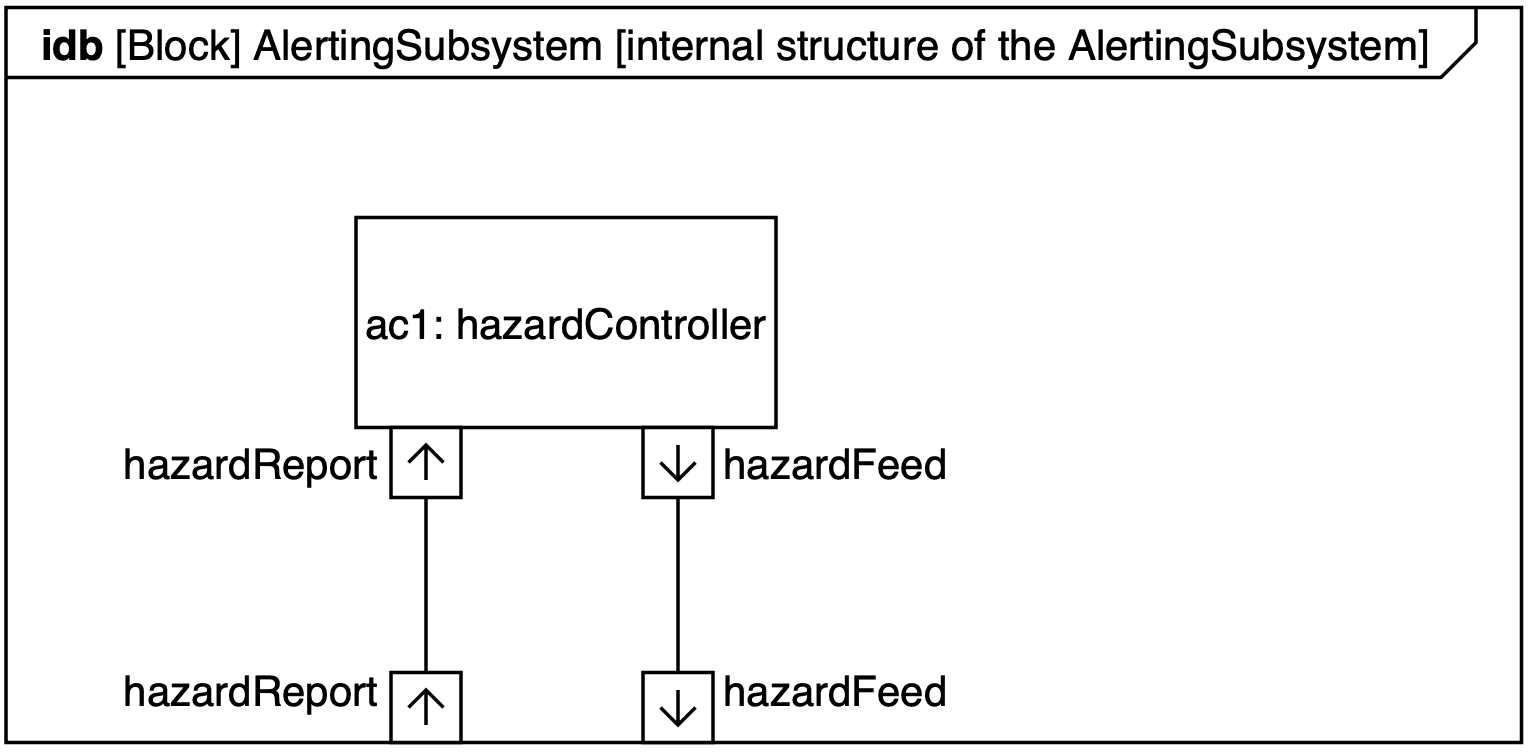
\includegraphics[width=\textwidth]{Internal_Block_Diagrams/IBD_Alerting.png}
  \caption{Internal Block Diagram: Alerting Subsystem}
  \label{fig:subsystems_alerting}
\end{figure}


\clearpage

\section*{Variability Model}
\subsection*{Feature Model}

\begin{figure}[H]
  \centering
  
\includegraphics[width=\textwidth]{imageS/feature_models/FeatureModel.png}
  \caption{Feature Model}
  \label{fig:featuremodel}
\end{figure}

\subsection*{Configurations}

\begin{figure}[H]
  \centering
  
\includegraphics[width=\textwidth]{imageS/feature_models/FeatureModelConfig1.png}
  \caption{Configuration 1}
  \label{fig:featuremodel}
\end{figure}

\begin{figure}[H]
  \centering
  
\includegraphics[width=\textwidth]{imageS/feature_models/FeatureModelConfig2.png}
  \caption{Configuration 2}
  \label{fig:featuremodel}
\end{figure}


\clearpage

\section*{Prototype}

\subsection*{Running Instructions}

\textbf{Backend:}
\begin{lstlisting}[language=bash]
cd msp-mywaze-backend
npm i
npm run dev
\end{lstlisting}

\textbf{Frontend:}
\begin{lstlisting}[language=bash]
cd msp-mywaze-frontend
npm i
npm run dev
\end{lstlisting}

The only prerequisites are a current version of \texttt{node} and \texttt{npm}. The database is implemented as SQLite, so no manual setup is necessary.

Routing uses OpenRouteService, which is quota-limited (daily) in the free version. If it stops working, please wait one day or change the variable \texttt{ORS\_API\_KEY} in \texttt{msp-mywaze-backend/src/routes/routing.ts} to your own (free) API key obtained from \url{https://openrouteservice.org}.

\subsection*{Features Implemented}

Screen recordings of all features can be found in the report/images/prototype directory, or in the readme file in the top level of the repository structure.

\subsubsection*{Basic Features}

\begin{itemize}
    \item \textbf{Registration}: User can register and login on the home page.
    \item \textbf{Vehicle Type Registration}: User can configure their vehicle type in the drop-down user menu on the top right of the screen.
    \item \textbf{Define Route}: User can define a route by entering the destination name or address into the text field at the top center and clicking \textit{Go}.
    \item \textbf{ETA}: ETA is displayed in a popup above the destination after a route is defined.
    \item \textbf{Speed Warning}: Current speed will turn red if the user moves over the speed limit. To test speed warnings on desktop, click on the speed value to generate a random speed around 50 km/h.
\end{itemize}

\subsubsection*{Advanced Existing Features}

\begin{itemize}
    \item \textbf{Bookmarking}: User can bookmark frequently used locations.
    \item \textbf{Hazard Reporting}: Users can report hazards encountered along the route. Reports are synchronized and shown across user sessions.
    \item \textbf{Recents}: Recently entered locations are shown for quick access.
    \item \textbf{Units}: Users can switch between metric and imperial units.
\end{itemize}

\subsubsection*{Advanced New Features}

\begin{itemize}
    \item \textbf{Stats}: Displays statistics for average speed, distance, and active days.
\end{itemize}

\end{document}